%file main.tex
%Adapted from
%http://yetanotherbiochemblog.wordpress.com/2011/10/11/managing-conference-materials-in-latex-part-1-abstract-template/
%Edited vss APRIL/2012

\documentclass[11pt,a5paper,twoside]{book}
\usepackage[a5paper]{geometry}
\usepackage[utf8x]{inputenc}
\usepackage[T1]{fontenc}
\usepackage[english]{babel}
\usepackage{fixltx2e}
\usepackage{hyphenat}
\usepackage[usenames,dvipsnames]{color}
%\usepackage{multicols}
\usepackage{longtable}




%a5 paper= 	148mm x 210mm
%a4 paper=	210mm x 297mm
\setlength\hoffset{-0.79cm} % 1
\setlength\oddsidemargin{0cm} % 3
\setlength\evensidemargin{0cm} % 3
\setlength\textwidth{110mm} % 8
\setlength\voffset{-2.54cm} % 2
\setlength\topmargin{1.1cm} % 4
\setlength\headheight{0.7cm} % 5
\setlength\headsep{0.4cm} % 6
\setlength\textheight{170mm} % 7
%\setlength\footskip{1.0cm} % 11
\parindent=0cm
\parskip=0.1cm

\renewcommand{\rmdefault}{ptm}

\newcommand{\anumber}[1]{\leavevmode{\textbf{#1}}}
\newcommand{\atitle}[1]{\leavevmode{\textbf{\large #1}}}
\newcommand{\affiliation}[1]{\leavevmode{\textit{#1}}}
\newcommand{\email}[1]{\leavevmode{\url{#1}}}
\newcommand{\presenting}[1]{\leavevmode{\textbf{\underline{#1}}}}
\newcommand{\authors}[1]{\textbf{\small #1}}

\usepackage{graphicx}
\usepackage{wrapfig}
\newcommand{\photo}[1]{
    \begin{wrapfigure}[4]{o}{0.2\textwidth}
    \includegraphics[width=0.2\textwidth]{#1}
    \end{wrapfigure}
}

\usepackage{fancyhdr}
\renewcommand{\headrulewidth}{0.2pt}
\renewcommand{\footrulewidth}{0.2pt}

\newcommand{\redefineheaders}[2]{
    \pagestyle{fancy}
    \fancyhf{}
    \fancyhead[L]{}
    \fancyhead[CO,CE]{}
    \fancyhead[R]{\small #2}
    \fancyfoot[R]{\thepage}
    \fancyfoot[CO,CE]{}
    \fancyfoot[L]{\textit{GRB 2012 - May 7-11, Munich, Germany}}
}

\usepackage{enumerate}

\usepackage{makeidx}
\makeindex

\begin{document}
\title{Abstracts}
\maketitle

\title{List of Participants}

\begin{multicols}{2}



\begin{center}
  \begin{tabular}{ l | c || r | }
    \hline
$LOP
    \hline
  \end{tabular}
\end{center}

\end{multicols}


\newpage

\redefineheaders{Monday, May 7}{Session I: Recent results from Swift and Fermi}
% $ABSTRACT_SESSION_I_1


\atitle{Swift: Status and Recent Results}

\bigskip

\authors{Judith Racusin}

\affiliation{NASA/GSFC}

\bigskip

\noindent After 7.5 years of operations and more than 700 detected GRBs, Swift continues to provide both surprises and insight into the Universe’s most exciting transient phenomena.  Swift operations remain efficient, including a new capability to more easily follow-up transients detected by other observatories.  In this talk, I will highlight recent GRB results that demonstrate Swift’s unique capabilities, and discuss potential areas of study in the future.

\index{\tiny{Racusin, Judith: \textit{Swift: Status and Recent Results}}}

% $ABSTRACT_SESSION_I_1


\atitle{Fermi LAT Status and Recent Results}

\bigskip

\authors{F. Piron, for the Fermi LAT Collaboration}

\affiliation{LUPM (CNRS/IN2P3 and Montpellier 2 University)}

\bigskip

\noindent The Fermi Large Area Telescope (LAT) is a pair-conversion detector of high-energy gamma rays of energies ranging from 20 MeV to more than 300 GeV. It operates in synergy with the Gamma-ray Burst Monitor (GBM), which covers the entire unocculted sky and is designed for gamma-ray transients' detection and spectroscopy between 8 keV and 40 MeV. The LAT detects $\sim$9 gamma-ray bursts (GRB) per year, which represents $\sim$8\% of the GBM bursts occuring in its field of view. We will present a systematic study of the GRB properties observed with the LAT, highlighting the unique characteristics of some individual bursts. We will also discuss the LAT non-detections of some GBM bright and hard bursts, in an effort to understand the difference in GRB rates from both instruments.

\index{\tiny{Piron, Frederic: \textit{Fermi LAT Status and Recent Results}}}

% $ABSTRACT_SESSION_I_1


\atitle{Scientific highlights from the Fermi Gamma-ray Burst Monitor}

\bigskip

\authors{Sheila McBreen on behalf of the GBM team}

\affiliation{University College Dublin}

\bigskip

\noindent The Fermi Gamma-ray Burst Monitor (GBM) is an all-sky instrument, sensitive in the 8 keV to 40 MeV energy range. GBM  detected over 900 Gamma-Ray Bursts (GRBs) in the four years since the launch of Fermi and the Large Area Telescope detected ~8% of those within the overlapping field of view. The spectral and temporal properties of the GBM GRB sample will be described. In addition to GRBs, GBM has triggered on other transient sources, such as soft gamma repeaters, terrestrial gamma-ray flashes and solar flares. I will discuss the performance, data products and scientific highlights of GBM.


\redefineheaders{Monday, May 7}{Session IIa: Prompt Emission Spectroscopy}
% $ABSTRACT_SESSION_IIa_2a


\atitle{The Fermi Era: Towards a better understanding of the GRB prompt emission}

\bigskip

\authors{sylvain Guiriec}

\affiliation{NASA Goddard Space Flight Center / ORAU}

\bigskip

\noindent Since 2008, prompt gamma-ray observations either by Fermi alone or jointly with Swift have changed our view of Gamma-Ray Bursts (GRBs). While Fermi data reproduce globally the results obtained a decade ago by CGRO from keV to GeV,the new capabilities enabled us to go much further, towards a better understanding of GRB emission mechanisms and of the GRB phenomenon overall.
In the Fermi Era, the empirical Band function, traditionaly-used to fit GRB spectra, is not the paradigm any more. Deviation from Band and possible identification of physical components are discussed in the litterature.
Through this presentation we will come back on the Fermi observations published in the literature and discuss how they support or challenge the various mechanisms proposed to explain the observed emission.

% $ABSTRACT_SESSION_IIa_2a


\atitle{Rest-frame properties of GRBs observed by Fermi/GBM}

\bigskip

\authors{D. Gruber on behalf of the GBM team.}

\affiliation{Max Planck Institute for Extraterrestrial Physics}

\bigskip

\noindent We present the main spectral and temporal properties of GRBs observed by Fermi/GBM. We investigate the key properties of GRBs in the rest-frame of the progenitor and test for possible intra-parameter correlations to better understand the intrinsic nature of these events.

Our sample comprises the 32 GRBs published by Gruber et al. 2011 together with all GBM GRBs with measured redshift found since August 2010 up to February 2012. For all of these events we derive $E_{\\rm p,rest}$, $T_{90,{\\rm rest}}$ and $E_{\\rm iso}$. We confirm the tight correlation between and $E_{\\rm p,rest}$ and $E_{\\rm iso}$ and the one between $E_{\\rm p,rest}$ and the 1-s peak luminosity ($L_p$). Moreover, we do not find any significant cosmic evolution of $E_{\\rm p,rest}$ or $T_{90,{\\rm rest}}$.

% $ABSTRACT_SESSION_IIa_2a


\atitle{Bright High-Energy GRBs detected with Fermi GBM}

\bigskip

\authors{Elisabetta Bissaldi}

\affiliation{UIBK}

\bigskip

\noindent We present the analysis of a sample of bright Gamma-Ray Bursts (GRBs) showing emission up to more than 1 MeV, which were collected during the first 3.5 years of Fermi Gamma-Ray Burst Monitor (GBM) operations.
We derive the durations of GRBs (T90) in the observer\'s frame in various energy bands up to 10 MeV, thus expanding the duration–energy relationship in the GRB light curves to high energies. Finally we compare our analysis with previous results.
For several bursts we notice evidence of a possible cutoff or break at higher energies in the duration vs. energy distributions and investigate this
behavior by relating it with the spectral properties of GRBs.

% $ABSTRACT_SESSION_IIa_2a


\atitle{Prompt spectral properties of a complete sample of Swift Gamma-Ray Bursts}

\bigskip

\authors{L. Nava}

\affiliation{APC Paris}

\bigskip

\noindent Thanks to Swift, rapid follow-up studies of GRBs are possible. About 1/3 of all GRBs observed by Swift has measured redshift (an enormous improvement with respect to the pre-Swift era). Salvaterra et al recently defined a subsample of Swift GRBs with 90\\% of redshift completeness, based on favorable observing conditions (Jakobsonn et al) and prompt brightness. We present their spectral properties and for the first time investigate the spectral-energy correlations in a sample unaffected by biases induced by the measurement of z. Using the complete sample as reference, we simulate samples of GRBs to probe the role of the flux threshold on the Ep-L relation. We found that the use of flux limited samples in correlation studies cannot be responsible for the existence of the correlation itself.

\index{\tiny{Nava, Lara: \textit{Prompt spectral properties of a complete sample of Swift Gamma-Ray Bursts}}}


\redefineheaders{Monday, May 7}{Session IIb: Prompt Emission Spectroscopy}
% $ABSTRACT_SESSION_IIb_2b


\atitle{Theory of the  Gamma-ray Burst Prompt Emission}

\bigskip

\authors{Davide Lazzati}

\affiliation{NCSU}

\bigskip

\noindent I will review the properties of the prompt emission in long and short duration gamma ray burst and the models that have been suggested to explain their features. I will discuss the pros and cons of each model and focus on recent theoretical developments suggesting that the long-GRB prompt emission comes from a combination of mechanisms, with photospheric radiation playing a key role. The implication of this for the short GRBs will be discussed.

% $ABSTRACT_SESSION_IIb_2b


\atitle{The Photosphere in Gamma-Ray Bursts: Lessons Learned from Fermi}

\bigskip

\authors{Felix Ryde}

\affiliation{Royal Insitute of Technology}

\bigskip

\noindent In spite of extensive research over the past decades, a complete physical picture of the origin of the prompt GRB emission is still lacking. The failure of the synchrotron interpretation raises the need for alternatives.  During recent years, though, evidence has been  accumulating that the jet photosphere plays an important role.   I will summarise the lessons learned from Fermi observations regarding the behaviour of the photosphere.  I will concentrate on a few strong and important bursts, namely, GRB090902, GRB100724A, and GRB110721A.   In particular, I will show evidence for sub-photospheric energy dissipation, and show how it can explain the non-thermal spectra seen in many bursts.  Finally, I will discuss some new ideas that may enable us to extract more information from Fermi data.

\index{\tiny{Ryde, Felix: \textit{The Photosphere in Gamma-Ray Bursts: Lessons Learned from Fermi}}}

% $ABSTRACT_SESSION_IIb_2b


\atitle{Photospheric Emission in Fermi Gamma Ray Bursts}

\bigskip

\authors{Sinead McGlynn}

\affiliation{Exzellenzcluster Universe Garching, MPE Garching}

\bigskip

\noindent We discuss the systematic time-resolved analysis of the brightest gamma-ray bursts observed by the Gamma ray Burst Monitor (GBM) on Fermi up to the end of 2011, where the prompt spectra show evidence for photospheric emission. We use the observed spectral parameters to determine the dynamics of the outflow in each burst. This extensive sample illustrates that photospheric emission may be present to a greater or lesser degree in each burst, depending on the level of subphotospheric dissipation present.

\index{\tiny{McGlynn, Sinead: \textit{Photospheric Emission in Fermi Gamma Ray Bursts}}}

% $ABSTRACT_SESSION_IIb_2b


\atitle{Single- and two-component gamma-ray burst spectra in the Fermi GBM-LAT energy range}

\bigskip

\authors{Péter Veres, Péter Mészáros}

\affiliation{Pennsylvania State University}

\bigskip

\noindent Most Fermi GRB spectra appear as either a broken power law extending to GeV energies or as a broken power with a separate GeV power law component. Here we show that such spectra can be understood in terms of magnetically dominated relativistic jets where a dissipative photosphere produces the prompt MeV emission, which is extended into the GeV range by inverse Compton scattering in the external shock, with possible contributions from a reverse shock as well. The bulk Lorentz factors required in these models are in the range of 300-600, and the MeV-GeV time delays arise naturally. In some cases an optical flash and a sub-dominant thermal component are also present.


\redefineheaders{Monday, May 7}{Session IIc: Prompt Emission Correlations and Temporal Properties}
% $ABSTRACT_SESSION_IIc_2c


\atitle{The Ep - Eiso relation: intrinsic GRB property or/and selection effects?}

\bigskip

\authors{R. Mochkovitch, R. Hascoet, F. Daigne, J.L. Atteia, S. Boci, M. Hafizi}

\affiliation{Institut d'Astrophysique de Paris}

\bigskip

\noindent Since its discovery the Ep - Eiso relation has been a source of controversy between those believing that it is an intrinsic GRB property, that should be directly related to the physics of the prompt emission and others, arguing that it comes from various selection effects (thresholds for burst and afterglow detection, conditions for measuring the redshift and peak energy). In the context of the internal shock model we present Monte-Carlo simulations showing that the observed relation may indeed result from a combination of intrinsic processes and selection effects. While at large Eiso we find that the relation can be interpreted in terms of the physics of internal shocks (which do not produce large Eiso - low Ep events), it appears largely shaped by selection effects at low Eiso.

\index{\tiny{Mochkovitch, Robert: \textit{The Ep - Eiso relation: intrinsic GRB property or/and selection effects?}}}

% $ABSTRACT_SESSION_IIc_2c


\atitle{GRBs have preferred jet opening angles and bulk Lorentz factors}

\bigskip

\authors{Ghisellini}

\affiliation{INAF - Osservatorio Astronomico di Brera}

\bigskip

\noindent We do not have a valid and robust explanation of the spectral energy correlations. Some light, however, have been shed by the recently found correlation between the bulk Lorentz factor and both the peak energy and the isotropic peak luminosity output of the prompt. Based on this result, we explore its consequences for the spectral energy correlations, finding, through extensive simulations, that they are real. Furthermore GRBs should be characterized by a preferred opening angle of their jets, and a preferred bulk Lorentz factor. These two quantities are related: the narrower the jet angle, the larger the bulk Lorentz factor.

% $ABSTRACT_SESSION_IIc_2c


\atitle{On the reliability of spectral-energy correlations in GRBs}

\bigskip

\authors{L. Amati [1], S. Dichiara [2], F. Frontera [2], C. Guidorzi [2]}

\affiliation{[1] INAF - IASF Bologna, [2] University of Ferrara}

\bigskip

\noindent The Ep,i - Eiso correlation, first reported by Amati et al. (2002), and other spectral-energy correlations derived from it are one of the most debated topics in GRB science, given their relevance for both GRB physics and cosmology. In particular, in the last years different research groups came to very different conclusions about the impact of selection and instrumental effects on these correlations. We give a critical review of these works and report the results of Monte Carlo simulations and the analysis of large datasets (CGRO/BATSE, BeppoSAX/GRBM, WIND/Konus, Swift/BAT, Fermi/GBM) that we performed in order to shade light on this important issue. We also discuss the reliability and perspectives of using spectral-energy correlations for measuring cosmological parameters up to z~9.

\index{\tiny{Amati, Lorenzo: \textit{On the reliability of spectral-energy correlations in GRBs}}}

% $ABSTRACT_SESSION_IIc_2c


\atitle{On The Lack of Time Dilation Signatures in Gamma-ray Burst Light Curves}

\bigskip

\authors{Daniel Kocevski}

\affiliation{Stanford University}

\bigskip

\noindent We present an analysis in which we examine the effects of time dilation on the temporal profiles of GRB pulses and the implications this has on our understanding of GRB energetics.  Through the use of simulations, we find that the observer frame duration of individual pulses does not increase with redshift as one would expect from cosmological expansion. Instead, the duration actually decreases as the pulse's signal-to-noise decreases with increasing redshift.  The results of our simulation are consistent with the fact that evidence for time dilation has not materialized in either the Swift or Fermi detected GRBs with known redshift.  We discuss how the measured durations and E$_{\rm iso}$ estimates for GRBs detected near the instrument's detection threshold should be considered as lower limits.

\index{\tiny{Kocevski, Daniel: \textit{On The Lack of Time Dilation Signatures in Gamma-ray Burst Light Curves}}}

% $ABSTRACT_SESSION_IIc_2c


\atitle{Energy-dependent Spectral Lags of Fermi-GBM GRBs}

\bigskip

\authors{S. Foley [1], P. N. Bhat [2], S. Guiriec [3] on behalf of the GBM team}

\affiliation{[1] School of Physics, University College Dublin, [2] CSPAR, University of Alabama in Huntsville, [3] NASA Goddard Space Flight Center}

\bigskip

\noindent The Fermi Gamma-ray Burst Monitor (GBM) has detected over 800 GRBs since its launch in June 2008. Many GRBs exhibit a spectral lag up to $\sim$1 MeV which is seen as high-energy gamma-ray emission arriving earlier than photons in a low-energy band. Here we present the spectral lags of a sample of bright and hard GBM GRBs with simple time profiles. The wide energy coverage of GBM (8 keV - 40 MeV) allows the dependence of the spectral lag on energies up to the MeV range to be investigated for bursts with sufficient signal in the BGO detectors. The relationship between the evolution of the spectral lag with energy and the spectral evolution of the burst is also investigated.

\index{\tiny{Foley, Suzanne: \textit{Energy-dependent Spectral Lags of Fermi-GBM GRBs}}}


\redefineheaders{Tuesday, May 8}{Session IId: Very High-Energy Emission}
% $ABSTRACT_SESSION_IId_2d


\atitle{Study of emission mechanism of Gamma-Ray Bursts by the gamma-ray polarization with IKAROS-GAP}

\bigskip

\authors{Daisuke Yonetoku [1], Toshio Murakami [2], Shuichi Gunji [2], Tatehiro Mihara [3], Kenji Toma [4], Tomonori Sakashita [1], Yoshiyuki Morihara [1], Takuya Takahashi [1], Noriyuki Toukairin [2], Hirofumi Fujimoto [1], Yoshiki Kodama [1]}

\affiliation{[1] Kanazawa University, [2] Yamagata University, [3] RIKEN, [4] Osaka University}

\bigskip

\noindent The Gamma-Ray Burst Polarimeter (GAP) aboard the solar sail IKAROS is the first polarimeter specifically designed to measure the gamma-ray polarization of prompt GRBs. We detected the polarization signals from three bright GRBs with almost above 3 sigma confidence level. For the case of GRB100826A, we also detected the firm change of polarization angle with 3.5 sigma confidence level. In view of gamma-ray polarization measurement, we consider that the magnetic fields may play an important role in the mechanism of prompt GRB. We suggest the non-axisymmetric (e.g. patchy) structures of the magnetic fields and/or brightness inside the relativistic jet within the observable angular scale of $\Gamma^{-1}$, to explain the observed significant change of polarization angle.

\index{\tiny{Yonetoku, Daisuke: \textit{Study of emission mechanism of Gamma-Ray Bursts by the gamma-ray polarization with IKAROS-GAP}}}

% $ABSTRACT_SESSION_IId_2d


\atitle{Broadband observations of GRB110731A with Fermi, Swift, GROND and MOA}

\bigskip

\authors{Johan Bregeon}

\affiliation{INFN Pisa}

\bigskip

\noindent We report on the multi-wavelength observations of the bright long GRB 110731A detected by Fermi and Swift, and follow-up observations by the MOA and GROND optical telescopes. The analysis of the prompt phase reveals that this GRB shares many features with the other bright bursts observed by Fermi-LAT during its first 3 years on-orbit. The wealth of multi-wavelength observations allowed
temporal and spectral analyses in different epochs, favoring emission from the forward shock in a wind-type medium. The temporally-extended emission observed by the LAT is most likely the highest-energy extension of the afterglow. Prompt emission from a single zone and forward shock afterglow analysis both lead independently to an estimated jet bulk Lorentz factor of Gamma~500.

% $ABSTRACT_SESSION_IId_2d


\atitle{GRB observations at very high energies with the MAGIC telescopes}

\bigskip

\authors{Markus Garczarczyk}

\affiliation{Instituto Astrofisica de Canarias}

\bigskip

\noindent Measurement of the GRB spectra and variability at the GeV range will constrain the ongoing physical processes of these phenomena. More than a decade ago, when the MAGIC telescope was in the design phase, the main goals were to build an IACT with the fastest repositioning speed and lowest energy threshold. These requirements are mandatory for measuring the VHE emission from GRBs. Currently MAGIC is a stereoscopic system of two telescopes operating at an energy threshold of few tens of GeV. The telescopes move to the opposite direction on the sky within less than 20 s. Follow-up observations are carried out with a frequency of ~10 events per year, however, without a significant detection until now. The MAGIC/LAT results and the modeling of the physical parameters of GRB090102 will be shown.

\index{\tiny{Garczarczyk, Markus: \textit{GRB observations at very high energies with the MAGIC telescopes}}}

% $ABSTRACT_SESSION_IId_2d


\atitle{Multi-GeV lightcurves: possible hints for the emission mechanism}

\bigskip

\authors{Katsuaki Asano [1], Peter Meszaros [2]}

\affiliation{[1] Tokyo Tech., [2] Penn. State}

\bigskip

\noindent Although the Fermi observatory has reported delayed onsets of GeV emissions, the photon statistic is not sufficient to distinguish the emission mechanisms. Future multi-GeV observations such as CTA may give us precise lightcurves that can be compared with lower energy bands. In this talk we show our time-dependent simulations for leptonic and hadronic models. Our results suggest that the multi-GeV lightcurves are powerful tool to probe the GeV emission mechanisms.

\index{\tiny{Asano, Katsuaki: \textit{Multi-GeV lightcurves: possible hints for the emission mechanism}}}


\redefineheaders{Tuesday, May 8}{Session IIIa: Afterglow Theory}
% $ABSTRACT_SESSION_IIIa_3a


\atitle{Scaling Properties of Afterglow Radiation}

\bigskip

\authors{Andrew MacFadyen and Hendrik van Eerten}

\affiliation{New York University}

\bigskip

\noindent I will present recent progress in calculating the dynamics of
afterglow jets and the electromagnetic transients they produce.  I
will demonstrate that the full dynamics, and even the light curves
themselves, can be arbitrarily scaled in energy and circumstellar
density. We have performed high-resolution two-dimensional
hydrodynamical calculations of afterglow jets with a range of initial
opening angle which can be scaled to fit broadband afterglow light curves
observed from arbitrary viewing angle.  The results of the simulations
are condensed into a few functions which we incorporate into an
iterative fitting code which will be available at
http://cosmo.nyu.edu/afterglowlibrary

\index{\tiny{MacFadyen, Andrew: \textit{Scaling Properties of Afterglow Radiation}}}

% $ABSTRACT_SESSION_IIIa_3a


\atitle{Multidimensional numerical simulations in the afterglow phase}

\bigskip

\authors{Alkiviadis Vlasis}

\affiliation{KU Leuven}

\bigskip

\noindent We present high resolution numerical simulations in 1D and 2D of two ultra-relativistic shells colliding in the afterglow phase of a GRB. For the 1D case we construct optical and radio light curves and examine the occurrence of flares assuming a spherical explosion and a hard-edged jet scenario. We establish a connection between the characteristics of the flare and the properties of the flow. For the 2D case we examine the propagation of a narrow 2 degrees half-opening angle jet and investigate the dynamical effects resulting from the energy injection in the external shell. We find an angular dependency of the collision time due to extraction of energy from the external shock and comment on the signatures this behaviour might have in optical light curves.

\index{\tiny{Vlasis, Alkiviadis: \textit{Multidimensional numerical simulations in the afterglow phase}}}

% $ABSTRACT_SESSION_IIIa_3a


\atitle{Relativistic MHD Simulations of Magnetic Fields in Jets of GRBs}

\bigskip

\authors{Gustavo Rocha da Silva, Diego Falceta-Gonçalves, Elisabete M. de Gouveia Dal Pino}

\affiliation{Universidade de São Paulo}

\bigskip

\noindent In all GRBs models, magnetic fields are important and play a very dramatic
role. In particular in the synchroton afterglow emission the downstream
magnetic field, implied by afterglow observations in GRBs, is higher than
that of the upstream field, by a factor \\sim $10^6$. Observations
indicates that the magnetic field in the downstream region must remain high
over distances $10^{10}$ \\delta, where \\delta is the plasma skin depth. In order to understand the behavior of magnetic fields in the evolution of the GRB jets, we have performed relativistic MHD (RMHD) simulations, taking into account the radiative losses to the external medium. Here we show the amplification of the magnetic fields by shock compression and how it is influenced by the cooling effects.

% $ABSTRACT_SESSION_IIIa_3a


\atitle{Simulations of GRB Jets in a Stratified External Medium: Dynamics, Afterglow Lightcurves, Jet Breaks and Radio Calorimetry}

\bigskip

\authors{Fabio De Colle}

\affiliation{University of California at Santa Cruz}

\bigskip

\noindent We present the first multi-dimensional simulations of the dynamics of GRB jets for both uniform and stratified external media. The simulations are performed in two dimensions using a newly developed, special relativistic, adaptive mesh refinement hydrodynamics code. 
We describe the differences in the dynamics of the GRB jet as a function of the stratification of the ambient medium and, by post-processing the results of the simulations with a radiation code, we compute the afterglow emission from the GRB as it decelerates from highly relativistic to Newtonian velocities. The implications for observations of the afterglow lightcurves, jet breaks and radio calorimetry are described in detail in the talk.

\index{\tiny{De Colle, Fabio: \textit{Simulations of GRB Jets in a Stratified External Medium: Dynamics, Afterglow Lightcurves, Jet Breaks and Radio Calorimetry}}}


\redefineheaders{Tuesday, May 8}{Session IIIb: Afterglow Observatons}
% $ABSTRACT_SESSION_IIIb_3b


\atitle{Observational Aspects of Gamma-ray Burst Afterglows}

\bigskip

\authors{Thomas Kruehler}

\affiliation{Dark Cosmology Centre}

\bigskip

\noindent For our understanding of the physics of GRB explosions as well as their implications on star formation and cosmology, it is crucial to observe the luminous afterglow emission. Afterglow observations provide an accurate distance scale to the GRB, and allow us to put constraints on the physical properties of the ultra-relativistic outflow. In the recent years, systematic follow-up campaigns have led to an increasing sample of high-quality afterglow light-curves and multi-wavelength SEDs. The new data sheds light on the properties of the population of long GRBs, including those events that have previously escaped detection.
I will give an overview of the state-of-the-art of the field and highlight new observational results.

\index{\tiny{Kruehler, Thomas: \textit{Observational Aspects of Gamma-ray Burst Afterglows}}}

% $ABSTRACT_SESSION_IIIb_3b


\atitle{Probing GRB afterglows with deep linear and circular polarimetry}

\bigskip

\authors{K. Wiersema}

\affiliation{University of Leicester}

\bigskip

\noindent Follow-up observations of large numbers of GRBs have produced a large sample of spectra and lightcurves, from which the basic micro- and macrophysical parameters of afterglows may be derived. However, a number of observed phenomena defy explanation by simple versions of the standard fireball model. Polarimetry can be a powerful diagnosis of (new) afterglow physics, probing the magnetic field properties and geometrical effects (e.g. jet breaks). 

We present the first high quality, multicolour, polarimetric curve of a Swift GRB afterglow, using the VLT. We obtained linear polarimetry in R band (0.13 - 2.3 days after burst) as well as K band, and deep circular polarimetry. We combine this unique dataset with multicolour lightcurves to probe models of jet breaks and magnetic field generation.

% $ABSTRACT_SESSION_IIIb_3b


\atitle{An intrinsic correlation between GRB optical/UV afterglow brightness and decay rate}

\bigskip

\authors{S. R. Oates [1], M. J. Page [1], P. Schady [2], M. De Pasquale [3]}

\affiliation{[1] MSSL, [2] MPE, [3] UNLV}

\bigskip

\noindent At this conference, I will provide evidence for a new intrinsic correlation between the decay rate and brightness of the optical afterglow, determined using a sample of 56 long GRB optical/UV light curves. This correlation has (at least) two possible origins: the energy is released more quickly for bright afterglows, or the energy is released at a similar rate in all afterglows, but we are observing the jets over a wide range of angles. In the latter scenario the fainter, slower-decaying afterglows will be viewed at larger angles than the brighter, faster-decaying afterglows. I will discuss these possible causes and the consequences on GRB afterglow physics. This correlation represents a major step towards toward a full, unified characterisation of the long GRB population.

% $ABSTRACT_SESSION_IIIb_3b


\atitle{The prompt-afterglow connection in Gamma-Ray Bursts: a comprehensive statistical analysis of Swift X-ray light-curves}

\bigskip

\authors{R. Margutti}

\affiliation{Harvard University}

\bigskip

\noindent I present a comprehensive statistical analysis of Swift X-ray light-curves of Gamma-Ray Bursts (GRBs), with more than 650 GRBs. Two questions drive this effort: Does the X-ray emission retain any kind of memory of the prompt phase? Where is the dividing line between long and short GRBs? I show that Short GRBs decay faster, are less luminous and less energetic than long GRB, but are characterized by very similar intrinsic absorption. I furthermore reveal the existence of a number of statistically significant relations that link the X-ray to prompt parameters in long GRBs; short GRBs are outliers of the majority of these 2-par relations. More importantly, I report on the existence of a universal 3-parameter scaling that links the X-ray and the gamma-ray properties of BOTH long and short GRBs

\index{\tiny{Margutti, Raffaella: \textit{The prompt-afterglow connection in Gamma-Ray Bursts: a comprehensive statistical analysis of Swift X-ray light-curves}}}


\redefineheaders{Tuesday, May 8}{Session IIIc: Afterglow Observations}
% $ABSTRACT_SESSION_IIIc_3c


\atitle{Gamma-ray burst afterglows as probes of the ISM}

\bigskip

\authors{Patricia Schady}

\affiliation{MPE Garching}

\bigskip

\noindent It has long been recognized that the bright and simple afterglow spectra of GRBs make highly effective probes of the ISM within distant, star-forming galaxies. Nevertheless, to fully exploit their potential, several outstanding issues need to be addressed. Most notably, the absorption imprint left on the X-ray afterglow from intervening material implies an order of magnitude more gas than is measured on optical spectra. I will present results from a comprehensive study on the multi-wavelength attenuation of GRB afterglows, and discuss the implied origin of the X-ray absorption excess. I shall also review current research on the extinction properties of host galaxy dust; a topic highly pertinent to optically `dark’ GRBs and to far-infrared/submm observations of host galaxy dust emission

% $ABSTRACT_SESSION_IIIc_3c


\atitle{Origin of the X-ray absorption in GRBs}

\bigskip

\authors{Darach Watson}

\affiliation{Dark Cosmology Centre}

\bigskip

\noindent The X-ray absorption in GRBs has been seen as a potential goldmine of information on material invisible at other wavelengths. Many proposals have been made to account for it, including ionisation of the GRB progenitor’s molecular cloud, intrinsic curvature of the X-ray spectra, and absorption by the warm-hot intergalactic medium.  However the correct solution to its origin has not been arrived at after more than a decade of work. I will present recent work on the X-ray absorption in GRBs that resolves the  problem of its apparent evolution with redshift by showing that a strong dust obscuration bias is responsible. I will then go on, using UV/optical data to suggest and demonstrate the solution to the remaining outstanding problems, and finally explain the nature of the X-ray absorber.

\index{\tiny{Watson, Darach: \textit{Origin of the X-ray absorption in GRBs}}}

% $ABSTRACT_SESSION_IIIc_3c


\atitle{Short GRB Broad-band Afterglow Observations: Beaming, Densities and Energetics}

\bigskip

\authors{Wen-fai Fong}

\affiliation{Harvard University}

\bigskip

\noindent While the progenitor model of long GRBs is widely accepted, the progenitors of short GRBs are not well understood. With potential gravitational wave detections a few years out, broad-band observations of short GRB afterglows provide essential information on the energetics and geometries of these events. Using X-ray, optical and radio data, I present the most current demographics of short GRBs in terms of their energies, circumburst densities and opening angles. I will then compare these observations to the rates we expect for various progenitor models.


\redefineheaders{Wednesday, May 9}{Session IVa: GRBs as Probes of the Early Universe}
% $ABSTRACT_SESSION_IVa_4a


\atitle{High-redshift Gamma-ray Burst Afterglows}

\bigskip

\authors{N. Tanvir}

\affiliation{University of Leicester}

\bigskip

\noindent The brightest GRB afterglows could, in principle, be seen at very high redshifts, during and before the epoch of reionization.  I will discuss the promise of GRB afterglows for pinpointing the locations of their faint host galaxies, and providing, via spectroscopy, information about their environments and the IGM that cannot be obtained by other means.  I will also review progress to-date in locating and studying GRB afterglows at very high-z, and consider prospects for the future.

\index{\tiny{Tanvir, Nial: \textit{High-redshift Gamma-ray Burst Afterglows}}}

% $ABSTRACT_SESSION_IVa_4a


\atitle{GRBs as standard  candles indicated by pulse spectral evolution}

\bigskip

\authors{Rupal Basak, A. R. Rao}

\affiliation{Tata Institute of Fundamental Research, Mumbai}

\bigskip

\noindent We analyze the time-resolved spectra of bright, long, single/separable pulses of Fermi GRBs. We find that the peak energy/temperature always decreases exponentially with fluence in the later part. We investigate multiple spectral components in the initial rising part and provide a comprehensive empirical description of the spectral and timing behavior of single pulses. We extend the work of Basak \& Rao (2012a ApJ745,76; 2012b ApJ, acc.) to make a pulse-wise parametrization of GRBs. We analyze all Fermi GRBs with known redshifts and demonstrate that the peak energy/kT at zero fluence shows a very strong correlation with the energy of  individual pulses. This work strongly extends the possibility of using GRB pulses as standard candles and the spectral parameters as a proxy for redshift.

\index{\tiny{Basak, Rupal: \textit{GRBs as standard  candles indicated by pulse spectral evolution}}}

% $ABSTRACT_SESSION_IVa_4a


\atitle{Difficulties in using GRBs as Standard Candles}

\bigskip

\authors{Adam Goldstein}

\affiliation{University of Alabama in Huntsville}

\bigskip

\noindent GRBs have been detected uniformly over the observable universe, ranging in comoving distance from a few hundred Mpc to a few thousand Mpc. For this reason there have been extensive studies into the possibility of using GRBs as standard candles. We discuss the attempts at defining GRBs as standard candles, such as the search for a robust luminosity indicator, pseudo-redshift predictions, the complications that emission collimation introduces into the estimation of the energetics, and the difficulty introduced by the widely varying observed properties of GRBs. These topics will be examined with data and analyses from both Fermi and Swift observations. Problems with current studies using GRBs as standard candles will be noted as well as potential paths forward to solve these problems.

% $ABSTRACT_SESSION_IVa_4a


\atitle{Galaxy counterparts of high-z sub-DLAs/DLAs towards GRBs}

\bigskip

\authors{Steve Schulze}

\affiliation{University of Iceland}

\bigskip

\noindent Until now, seven intervening sub-DLAs and DLAs have been reported towards six GRBs. Although their chemical composition and frequency is known from quasar studies, the knowledge of their galaxy counterparts is limited. In this talk, I present the findings on the first systematic search for galaxy counterparts of intervening sub-DLAs/DLAs towards GRBs. To identify their galaxy counterparts, very deep imaging campaigns and low-resolution spectra were used. This approach allowed the identification of one high-z DLA galaxy. I also discuss the limits on the non-detections and report a redshift co-incidence of different objects associated with metal-lines in the same field that are separated by 137-161 kpc.


\redefineheaders{Wednesday, May 9}{Session IVb: GRBs as Probes of the Early Universe}
% $ABSTRACT_SESSION_IVb_4b


\atitle{Gamma-ray Bursts as Probes of the First Stars}

\bigskip

\authors{Volker Bromm}

\affiliation{University of Texas at Austin}

\bigskip

\noindent I will review the basic theoretical framework for the formation of the first stars and galaxies. High-redshift gamma-ray bursts are among the most promising probes of this crucial epoch of first light. We will learn about the properties of individual first star progenitors, the cosmic star formation rate at high redshifts, and the ionization structure and metal enrichment of the early intergalactic medium.

\index{\tiny{Bromm, Volker: \textit{Gamma-ray Bursts as Probes of the First Stars}}}

% $ABSTRACT_SESSION_IVb_4b


\atitle{Pop III GRBs: constraints on the event rate for future surveys}

\bigskip

\authors{Rafael S. de Souza [1,2], Naoki Yoshida [3], Kunihito Ioka [4]}

\affiliation{[1] USP, [2] MPA, [3] IPMU, [4] KEK}

\bigskip

\noindent We calculate the theoretical event rate of gamma-ray bursts (GRBs)  from the collapse of massive first-generation stars (Pop III). The Pop III GRBs could be super-energetic, providing a unique probe of the high-redshift Universe. We employ a semi-analytical approach that considers inhomogeneous hydrogen reionization and chemical evolution of the intergalactic medium. We also discuss the best strategies to observe and identify these objects.

% $ABSTRACT_SESSION_IVb_4b


\atitle{The long gamma-ray burst rate and the correlation with host galaxy properties}

\bigskip

\authors{J. Elliott [1], J. Greiner [1], S. Khochfar [1], P. Schady [1], J. L. Johnson [1,2], A. Rau [1]}

\affiliation{[1] MPE Garching, [2] Los Alamnos Laboratory}

\bigskip

\noindent The association of long gamma-ray bursts (LGRB) with the death of massive stars allows the cosmic star formation history (CSFH) to be probed to higher redshifts than current conventional methods, however, no consensus on the manner in which the LGRB rate traces the CSFH has been reached. Driven by recent highly complete LGRB samples, obtained by GROND over the past 4 years, and new evidence of LGRBs occuring in more massive and metal rich galaxies than previously thought, the possible biases of the LGRBR-CSFH connection are investigated over a large range of galaxy properties. It is found that there is no strong preference for a metallicity cut or fixed galaxy mass boundaries and that there are no unknown redshift effects, in contrast to previous work.

% $ABSTRACT_SESSION_IVb_4b


\atitle{Probing Cosmic Radiation Fields and Magnetic Fields in the Reionization Epoch with Hard X-rays and MeV-GeV Gamma Rays from High-z GRBs}

\bigskip

\authors{Susumu Inoue [1], Yoshiyuki Inoue [2], Masakazu A. R. Kobayashi [3], Tomonori Totani [2], Keitaro Takahashi [4], Kiyotomo Ichiki [5]}

\affiliation{[1] ICRR, U. Tokyo, [2] Kyoto U., [3] NAOJ, [4] Kumamoto U., [5] Nagoya U.}

\bigskip

\noindent The extragalactic background light (EBL) in the rest-frame UV plays a crucial role during cosmic reionization. Based on semi-analytic models of galaxy formation, we develop a model of the EBL for z=0-10 that include Pop III stars and are consistent with current reionization constraints from QSO spectra and CMB polarization. The EBL can be probed via attenuation features due to gamma-gamma interactions in the 10-100 GeV spectra of high-z GRBs. Furthermore, the electron-positron pairs produced in such interactions can induce delayed secondary emission by scattering the CMB up to hard X-ray to multi-MeV energies, which provide a unique probe of intergalactic magnetic fields as well as the EBL during reionization. We discuss the observational prospects for CTA, ASTRO-H and other instruments.


\redefineheaders{Thursday, May 10}{Session Va: Progenitors of Long Duration Bursts}
% $ABSTRACT_SESSION_Va_5a


\atitle{The supernovae of gamma-ray bursts}

\bigskip

\authors{David Bersier}

\affiliation{Liverpool John Moores University}

\bigskip

\noindent The connection between long GRBs and supernovae is now well established. I will review the evidence in favor of - or against - it. I will attempt to separate solid facts from  weak evidence, interesting clues from red herrings. I will also look at what we  can learn from looking at SNe not associated with GRBs and see how GRBs fit into the broad picture of stellar explosions.

% $ABSTRACT_SESSION_Va_5a


\atitle{Collapsar and Magnetar Models for Long-Duration Gamma-Ray Bursts}

\bigskip

\authors{Shigehiro NAGATAKI}

\affiliation{Yukawa Institute for Theoretical Physics, Kyoto Univeristy}

\bigskip

\noindent I would like to review the numerical study on the central engine of Long-Duration Gamma-Ray Bursts (LGRBs). Mainly I would like to review the history and current status of collapsar model and magnetar model. I would like to present my numerical simulations of collapsar model using 2D/3D Generala Relativistic MHD code. I would like to explain Blandford-Znajek Process as a possible key process of the engine of LGRBs. I would also like to show our 2D MHD simulations of magnetar model.

% $ABSTRACT_SESSION_Va_5a


\atitle{Binary Progenitors for Long-Duration Gamma-Ray Bursts}

\bigskip

\authors{Philipp Podsiadlowski}

\affiliation{Oxford University}

\bigskip

\noindent In this talk I review recent progress on binary progenitor models for
long-duration gamma-ray bursts, involving tidal spin-up models, merger
models and explosive common-envelope ejection. Most of these models
require a late binary interaction (so-called Case C mass transfer) and
work better at lower metallicity. However, unlike some popular
single-star models, this is not required and may prove to be an
important discriminant. Indeed, this is
consistent with recent evidence that LGRBs do not avoid high-Z host galaxies.  Estimates for the various channels are consistent with an estimated LGRB rate of $\\sim 10^{-5}\\,$yr$^{-1}$ in
a typical galaxy, in particular, if the newly recognized mode of Case
D mass transfer contributes to the LGRB rate.

% $ABSTRACT_SESSION_Va_5a


\atitle{Long gamma-ray bursts from interacting binaries}

\bigskip

\authors{Ross Church [1], Melvyn Davies [1], Andrew Levan [2], Chunglee Kim [3]}

\affiliation{[1] Lund University, [2] University of Warwick, [3] West Virginia University}

\bigskip

\noindent The origin of long-duration gamma-ray bursts in the core-collapse of
rapidly-rotating massive stars is well supported by observations. However, it is difficult to prevent the progenitor's spin being braked by strong winds on the main sequence.  This prevents the post-core-collapse accretion disc forming.  The problem is worsened by recent observations of long gamma-ray bursts in high-metallicity regions.  I will show that, in a close binary, it is possible to replenish the spin of the star's core using tides to extract angular momentum from the binary's orbit.  This mechanism requires the progenitor to be in a close binary with a black hole.  I will show that this scenario naturally predicts features in the accretion history that can be tested using light curves of long gamma-ray bursts.

\index{\tiny{Church, Ross: \textit{Long gamma-ray bursts from interacting binaries}}}


\redefineheaders{Thursday, May 10}{Session Vb: Progenitors of Short Duration Bursts}
% $ABSTRACT_SESSION_Vb_5b


\atitle{The multi-messenger picture of compact binary mergers}

\bigskip

\authors{S.Rosswog}

\affiliation{Jacobs University Bremen}

\bigskip

\noindent The merger of compact binary systems are generally considered as the standard
central engines of sGRBs, but this hypothesis is far from being proven.
Progress is expected from combining the information obtained in different channels.
I will discuss the signatures extracted from a large set of simulated compact binary
mergers. They include gravitational waves and neutrinos, but the main focus will be
on the electromagnetic signatures that result from the dynamically ejected
matter. I will also discuss the potential of dynamical collisions of compact objects
as sGRB engines and the question in which ways such collisions differ from
gravitational wave driven mergers.

\index{\tiny{Rosswog, Stephan: \textit{The multi-messenger picture of compact binary mergers}}}

% $ABSTRACT_SESSION_Vb_5b


\atitle{Energy injection in short GRBs and the role of magnetars}

\bigskip

\authors{A. Rowlinson [1], P.T. O'Brien [2]}

\affiliation{[1] University of Amsterdam, [2] University of Leicester}

\bigskip

\noindent A significant fraction of the Long Gamma-ray Bursts (GRBs) in the Swift sample show a plateau phase which may be due to ongoing energy injection. We find many Short GRBs detected by the Swift satellite show similar behavior. The remnant of NS-NS mergers may not collapse immediately to a BH (or even collapse at all) forming instead a magnetar. This model predicts that there would be a plateau phase in the X-ray lightcurve followed by a shallow decay phase, if it is a stable magnetar, or a steep decay if the magnetar collapses to a BH. By fitting this model to all of the Short GRB BAT-XRT lightcurves, we find that a significant fraction may show evidence of energy injection by a magnetar. This model can be tested using the next generations of gravitational wave observatories.

\index{\tiny{O\'Brien, Paul: \textit{Energy injection in short GRBs and the role of magnetars}}}

% $ABSTRACT_SESSION_Vb_5b


\atitle{Model of the extended emission of short gamma-ray bursts}

\bigskip

\authors{Alexei Pozanenko [1], Maxim Barkov [2,1]}

\affiliation{[1] Space Research Institute, [2] Max-Planck-Institut fur Kernphysik}

\bigskip

\noindent The existence of extended emission (EE) is an intriguing property of short-duration gamma-ray bursts: the nature of the EE is still unclear. We consider short gamma-ray bursts, emphasizing the common properties of both short bursts and short bursts with EE. We propose a two jet model which can describe both short main episode of hard spectra emission, specific for short bursts, and softer spectra EE by different off axis position of observer. The model involves a short-duration jet, which is powered by heating due to neutrino annihilation, and a long-lived Blandford–Znajek jet with a significantly narrow opening angle. The model is a plausible mechanism for short-duration burst energization. It can explain short bursts both with and without EE within a single class of progenitor

\index{\tiny{Pozanenko, Alexei: \textit{Model of the extended emission of short gamma-ray bursts}}}

% $ABSTRACT_SESSION_Vb_5b


\atitle{Poster Prize Session}

\bigskip

\authors{Arne Rau}

\affiliation{MPE Garching}

\bigskip

\noindent Announcement of the poster price winners

\index{\tiny{Rau, Arne: \textit{Poster Prize Session}}}


\redefineheaders{Thursday, May 10}{Session Vc: Central Engine Physics}
% $ABSTRACT_SESSION_Vc_5c


\atitle{GRB central engine, jet formation and propagation}

\bigskip

\authors{Ehud Nakar}

\affiliation{Tel Aviv University}

\bigskip

\noindent The requirements from a GRB central engine are extreme: ejection of highly luminous, narrowly collimated, relativistic jets. The jet variability time scale is milliseconds, while the engine must be active for seconds to minutes and possibly even hours. I will first discuss the two popular engine models, accreting black-hole and proto-magnetar, and the constraints that they impose on the progenitor system of both long and short GRBs.  I will then focus on the Collapsar model for long GRBs and on the interaction of a relativistic jet with a stellar envelope. I will show that this interaction leaves an observed signature, which is detectable in the GRB samples of all major satellites, and discuss what can be learned from this signature on the typical GRB engine activity time.

\index{\tiny{Nakar, Ehud: \textit{GRB central engine, jet formation and propagation}}}

% $ABSTRACT_SESSION_Vc_5c


\atitle{Constraints to the GRB central engine from jet penetrability to massive stars}

\bigskip

\authors{Hiroki Nagakura, Yudai Suwa, Kunihito Ioka}

\affiliation{Kyoto University}

\bigskip

\noindent We numerically investigate jet propagation in various types of massive GRB progenitors and try to constrain to the nature of the central engine. In this study, two dimensional axisymmetric simulations of relativistic hydrodynamics are performed with taking into account both the stellar collapse and the jet propagation. In our simulations, the power of jet is determined by two different origin of central engine (accretion-powered central engine and neutrino-driven central engine). We calculate the accretion rate and the evolution of black hole mass and spin, all of which are necessary to evaluate the jet power. In this conference, I would like to show you a simple jet breakout criteria and also give constraints on the angular momentum distribution of Wolf-Rayet stars to produce GRBs.

% $ABSTRACT_SESSION_Vc_5c


\atitle{Unveiling long lasting central engine activity with Optical-NIR afterglows}

\bigskip

\authors{Marco Nardini [1], Jochen Greiner [2]}

\affiliation{[1] Università degli studi Milano-Bicocca, [2] MPE Garching}

\bigskip

\noindent In the standard view describing the nature of long GRB emission, the duration of the central engine activity has been usually considered to be 
much shorter that the afterglow emission variability time-scales.
The discussion on the nature of X-ray flares and the recent studies on pre and post cursor emission observed in the gamma rays unveiled the possibility that the central engine can be characterized by a much longer activity. In this work we discuss the signatures of late-time central engine activity from a different perspective, i.e., in the temporal and spectral variability of the optical-NIR afterglow. We will discuss these signatures of the long lasting central engine activity unveiled thanks to the rich multicolor light-cureves obtained by the GROND instrument.

\index{\tiny{Nardini, Marco: \textit{Unveiling long lasting central engine activity with Optical-NIR afterglows}}}

% $ABSTRACT_SESSION_Vc_5c


\atitle{Unifying Black Hole Jets in AGNs and GRBs}

\bigskip

\authors{R. S. Nemmen [1], M. Georganopoulos [2], S. Guiriec [1], E. Meyer [3], N. Gehrels [1], R. M. Sambruna [4]}

\affiliation{[1] NASA GSFC, [2] UMBC, [3] Rice, [4] George Mason University}

\bigskip

\noindent The central engines of AGNs and GRBs share the same basic astrophysical ingredients - despite the vastly different mass scales - and an outstanding question is how the jet physics scales from GRBs to AGNs. Using Fermi and Swift, we show that the jets produced by blazars and long-duration GRBs exhibit similar correlations between the kinetic power and apparent gamma-ray luminosity. After beaming corrections, we find evidence that blazars and GRBs follow the same correlation between the *intrinsic* Lgamma and kinetic power. This result implies that jet production and energy dissipation mechanisms are remarkably similar across 9 orders of magnitude in luminosity. We will discuss the implications of these results in terms of the properties of the central engines.


\redefineheaders{Thursday, May 10}{Session VI: History and Future Instrumentation}
% $ABSTRACT_SESSION_VI_6


\atitle{The Initial Gamma Ray Transient Studies}

\bigskip

\authors{Thomas L. Cline}

\affiliation{Goddard Space Flight Center, Emeritus}

\bigskip

\noindent The early studies of astronomical gamma ray transients are reviewed, with emphasis on our involvements and related developments, e.g., the first gamma ray burst detections and the creation of the Interplanetary Network. I interpreted the 1979 March 5 event as unique, whereas this initial IPN success appeared to ironically complicate and deepen the mystery of GRBs, with other views that its N49 snr id. was accidental or that it suggested nearby n-star origins. Other early experiments are outlined, e.g. our Shuttle Gamma-Dome that inspired the CGRO-BATSE, the Ge GRB spectrometer, and the Solar Polar Mission, reduced to the successful but no longer stereoscopic Ulysses. Other developments prior to the cosmological GRB era, e.g. the resolution of the magnetar/GRB confusion, are outlined.

\index{\tiny{Cline, Thomas: \textit{The Initial Gamma Ray Transient Studies}}}

% $ABSTRACT_SESSION_VI_6


\atitle{The History and Legacy of BATSE}

\bigskip

\authors{Gerald J. (Jerry) Fishman}

\affiliation{NASA-Marshall Space Flight Center}

\bigskip

\noindent The BATSE experiment on the Compton Gamma-ray Observatory was the first large detector system specifically designed for the study of gamma-ray bursts. The eight large-area detectors allowed full-sky coverage and were optimized to operate in the energy region of the peak emission of most GRBs.  BATSE provided detailed observations of the temporal and spectral characteristics of large samples of GRBs, and it was the first experiment to provide rapid notifications of the coarse location of many them.  It also provided strong evidence for the cosmological distances to GRBs through the observation of the sky distribution and intensity distribution of numerous GRBs.  The origin and development of the BATSE experiment, some highlights from the mission and its continuing legacy will be described.

% $ABSTRACT_SESSION_VI_6


\atitle{The Interplanetary Network Database}

\bigskip

\authors{Kevin Hurley, on behalf of all the Interplanetary Network team members, 1990 - present}

\affiliation{UC Berkeley Space Sciences Laboratory}

\bigskip

\noindent The Interplanetary Network Database, at ssl.berkeley.edu/ipn3, is composed of three main sections.
1.	A GRB bibliography containing over 11000 references from 1972 to the present, updated roughly every day,
2.	A master list of gamma-ray and SGR bursts with over 25000 events from 1990 to the present, updated roughly every month, and
3.	A table of over 7000 GRB localizations from 1990 to the present, updated roughly daily.
A detailed description of each of these sections is given, with indications of how to use the various datasets, and descriptions of the projects which are now underway to simplify web access to the localization data.

% $ABSTRACT_SESSION_VI_6


\atitle{Cosmic gamma-ray bursts studies with Ioffe Institute Konus experiments}

\bigskip

\authors{R.L. Aptekar, S.V. Golenetskii, D.D. Frederiks, E.P. Mazets, V.D. Pal'shin}

\affiliation{Ioffe Physico-Technical Institute, St. Peresburg, Russian Federation}

\bigskip

\noindent We present a short review of GRB studies being performed for many years by Ioffe Institute onboard a number of space missions. The first breakthrough in the studies of GRB was made possible by four Konus experiments carried out by the Ioffe Institute onboard the Venera 11 to 14 deep space missions in 1978 to 1983. A new important stage of our research  is associated with joint Russian-American experiment with the Russian Konus scientific instrument onboard the U.S. Wind spacecraft which has been successfully operating since its launch in November 1994. The Konus-Wind experiment has made an impressive number of important GRB observations and other astrophysical discoveries, due to the advantages of its design and its interplanetary locations. We also discuss our future GRB experiments.

\index{\tiny{Aptekar, Rafail: \textit{Cosmic gamma-ray bursts studies with Ioffe Institute Konus experiments}}}

% $ABSTRACT_SESSION_VI_6


\atitle{GRB experiments on-board of "Lomonosov" satellite}

\bigskip

\authors{Anatoli Iyudin, on behalf of "Lomonosov" collaboration}

\affiliation{Moscow State University, Skobeltsyn Institute of Nuclear Physics}

\bigskip

\noindent Russian satellite "Lomonosov" dedicated to the 300-year jubileum of M.V. Lomonosov, the great Russian scientist and founder of Moscow State University, is planned to be launched at fall 2012. The instrumentation on-board contain few of GRB dedicated units to study the prompt emission and afterglow at different wavelengths, including optical, UV, X-rays and gamma-rays. Science goals and means to achieve those will be given in this presentation.

\index{\tiny{Iyudin, Anatoli: \textit{GRB experiments on-board of "Lomonosov" satellite}}}

% $ABSTRACT_SESSION_VI_6


\atitle{Observing transients with LOFAR and AARTFAAC}

\bigskip

\authors{A. Rowlinson on behalf of the LOFAR Transients Key Project}

\affiliation{University of Amsterdam}

\bigskip

\noindent The Low Frequency Array (LOFAR) is a new European radio telescope operating at 30-240 MHz. LOFAR will offer an exciting opportunity to study the radio emission from GRBs at timescales from first detection until years afterwards. I will describe the features LOFAR will be able to use to study GRBs including:
1. Dedicated and commensal real-time monitoring programmes enabling detection and monitoring of radio afterglows.
2. Rapid, automated response to targets of opportunity.
3. A raw data buffer, providing the ability to "re-observe" past events at high time, spectral and spatial resolution.
4. Rapidly sharing newly detected transients using VOEvents.
Additionally, the AARTFAAC Project will build upon the core LOFAR capabilities to provide an all-sky real time monitor for bright transients.

\index{\tiny{Rowlinson, Antonia: \textit{Observing transients with LOFAR and AARTFAAC}}}

% $ABSTRACT_SESSION_VI_6


\atitle{Hunting for Gamma Ray Bursts with Pi of the Sky telescopes in Chile and Spain}

\bigskip

\authors{M.Siudek et al. (Pi of the Sky Collaboration)}

\affiliation{Center for Theoretical Physics PAS}

\bigskip

\noindent Pi of the Sky is a system of  wide field-of-view  robotic telescopes, which search for short timescale astrophysical phenomena, especially for prompt optical GRB emission. The system was designed for autonomous operation, following the predefined observation strategy and adopting it to the actual conditions. Simultaneous observations from locations in Chile and Spain allows for a systematic search of optical transients of cosmological origin.
Accurate analysis of data arising from a wide-field system like Pi of the Sky  is a real challenge because of a number of factors that can influence measurements. We have developed a set of dedicated algorithms which remove poor quality measurements, improve photometric accuracy and allow us to reach uncertainties  as low as 0.015 – 0.02 mag.

\index{\tiny{Siudek, Malgorzata: \textit{Hunting for Gamma Ray Bursts with Pi of the Sky telescopes in Chile and Spain}}}


\redefineheaders{Friday, May 11}{Session VII: Grav. Waves, Neutrinos, Cosmic Rays and UHE Emission}
% $ABSTRACT_SESSION_VII_7


\atitle{GRBs at Neutrino Telescopes}

\bigskip

\authors{Markus Ahlers}

\affiliation{UW Madison}

\bigskip

\noindent Gamma ray bursts are among the prime suspects as the sources of ultra-high energy (UHE) cosmic rays (CRs). Not only are these objects capable of accelerating nuclei to the extreme energies so far detected but they can also supply enough power to sustain the energy density of UHE CRs. The acceleration of nuclei in the source in the presence of radiation fields from the burst or afterglow leads immediately to the production of high energy neutrinos. I will review the expected neutrino fluxes in the standard GRB fireball model. I will show that the IceCube neutrino observatory has now reached the sensitivity to test these fluxes and challenges the UHE CR paradigm of GRBs.

\index{\tiny{Ahlers, Markus: \textit{GRBs at Neutrino Telescopes}}}

% $ABSTRACT_SESSION_VII_7


\atitle{Neutrinos from GRBs, and the connection to gamma-ray observations}

\bigskip

\authors{Philipp Baerwald, Svenja Hümmer, Walter Winter}

\affiliation{Universität Würzburg}

\bigskip

\noindent The possibility of GRBs as the source of UHECR is currently starting to get constrained by the non-observation of GRB neutrinos. We therefore reconsider the current neutrino flux predictions
from gamma-ray observations, based on the internal shock model, from the particle physics involved, and numerically calculate the resulting spectra. At the example of the Waxman-Bahcall GRB neutrino flux we demonstrate how additional production modes, synchrotron cooling of secondary particles, and flavor mixing affect the expected neutrino spectrum. We demonstrate that a detailed (numerical) calculation changes the prediction of the GRB neutrino flux from gamma-ray observations, apply this to the recent IC40 GRB results, and discuss systematical and astrophysical uncertainties of this interpretation.

% $ABSTRACT_SESSION_VII_7


\atitle{Gravitational Waves from Gamma-ray Bursts}

\bigskip

\authors{Alessandra Corsi}

\affiliation{California Institute of Technology}

\bigskip

\noindent tbd

\index{\tiny{Corsi, Alessandra: \textit{Gravitational Waves from Gamma-ray Bursts}}}

% $ABSTRACT_SESSION_VII_7


\atitle{The Swift short gamma-ray burst rate density: implications for detecting neutron star mergers by ALIGO}

\bigskip

\authors{David Coward [1], Eric Howell [1], Tsvi Piran [2], Giulia Stratta [3], Marica Branchesi [4], Omer Bromberg [3], Bruce Gendre [4], Ronald Burman [1], Dafne Guetta [5]}

\affiliation{[1] School of Physics, University of Western Australia, [2] Racah Institute of Physics, The Hebrew University, [3] ASI Science Data Center, [4] DiSBeF - Universita degli Studi di Urbino `Carlo Bo', [5] Department of Physics and Optical Engineering, ORT Braude}

\bigskip

\noindent Presently there are only some 30% of short gamma ray bursts (SGRBs) with reasonably firm redshifts, and this sample is highly biased by the limited sensitivity of Swift to detect SGRBs. We account for the dominant biases to calculate a realistic SGRB rate density out to z = 0.5 using the Swift sample of peak fluxes, redshifts, and those SGRBs with a beaming angle constraint from X-ray/optical observations. Assuming a significant fraction of binary neutron star mergers produce SGRBs, we calculate lower and upper detection rate limits of (1-200) per Yr by an ALIGO and Virgo coincidence search. Our detection rate is similar to the lower and realistic rates inferred from extrapolations using Galactic pulsar observations and population synthesis.

\index{\tiny{Coward, David: \textit{The Swift short gamma-ray burst rate density: implications for detecting neutron star mergers by ALIGO}}}


\redefineheaders{Friday, May 11}{Session VIII: Host Galaxies}
% $ABSTRACT_SESSION_VIII_8


\atitle{TOUGH: Observational Aspects of Gamma-ray Burst Host Galaxies}

\bigskip

\authors{Jens Hjorth}

\affiliation{Dark Cosmology Centre, Niels Bohr Institute, University of Copenhagen}

\bigskip

\noindent I give a brief review of what we know about GRB-selected galaxies. The heterogeneous nature of this population of galaxies highlights the fact that careful selection is a prerequisite for studying their statistical properties. I introduce The Optically Unbiased GRB Host (TOUGH) sample of 69 Swift GRB host galaxies spanning the redshift range 0.03-6.30 and announce the  results of a large observational survey of these galaxies.

\index{\tiny{Hjorth, Jens: \textit{TOUGH: Observational Aspects of Gamma-ray Burst Host Galaxies}}}

% $ABSTRACT_SESSION_VIII_8


\atitle{Gamma-ray Burst Host Galaxies as Probes of Galaxy Formation and Evolution}

\bigskip

\authors{Emily Levesque}

\affiliation{University of Colorado at Boulder}

\bigskip

\noindent Host galaxies are an excellent means of probing the natal environments that generate gamma-ray bursts (GRBs). Surveys of long-duration GRB (LGRB) host environments and their ISM properties have produced intriguing new results with important implications for LGRB progenitor models. These host studies are also critical in evaluating the utility of LGRBs as potential tracers of star formation and metallicity at high redshifts, particularly when considering the implications for properties of host galaxies above z = 6. I will summarize the latest research on LGRB host galaxies, and discuss the resulting impact on our understanding of these events: progenitors, energetics, afterglow properties, and cosmological applications.

\index{\tiny{Levesque, Emily: \textit{Gamma-ray Burst Host Galaxies as Probes of Galaxy Formation and Evolution}}}

% $ABSTRACT_SESSION_VIII_8


\atitle{The Host Galaxies of Dust-Obscured Gamma-Ray Bursts}

\bigskip

\authors{Daniel Perley}

\affiliation{Caltech}

\bigskip

\noindent I will present the latest observations from major programs on Spitzer, HST, Keck, and Gemini targeting the hosts of over 20 GRBs with highly dust-suppressed afterglows, as well as efforts to search for long-wavelength host emission using the EVLA and CSO.  Many dark GRB hosts are extremely red and IR-luminous, suggesting that GRBs can indeed form in massive and metal-enriched systems, bolstering their utility as a cosmic SFR probe and imposing important constraints on the progenitor.  However, radio/submillimeter observations indicate they are mostly not super-starbursting galaxies like local ULIRGs.  Many other dark GRB hosts are actually quite blue and have low stellar masses, confirming that even ordinary and seemingly dust-free systems can host significant obscured star formation.

\index{\tiny{Perley, Daniel: \textit{The Host Galaxies of Dust-Obscured Gamma-Ray Bursts}}}

% $ABSTRACT_SESSION_VIII_8


\atitle{The Italian-French X-shooter GRB host program: status and updates}

\bigskip

\authors{S.D. Vergani on behalf of the Italian-French X-shooter collaboration}

\affiliation{INAF-OAB}

\bigskip

\noindent The Italian-French GRB host program is one of the X-shooter GTO programs. It started at the end of 2009 and allowed us to collect the spectra of about 30 host galaxies in the 300-2400nm range from a redshift of about z=0.1 to z=2.7. In this talk I will present the status of the program, showing some of the new results obtained in both slit and IFU modes.


\newpage %Make a nice poster session cover page?

\redefineheaders{}{P-II: Prompt and High-Energy Emission}
% $POSTERS_SESSION_PII_p2
P-II-1

\atitle{Variation of the Rest-Frame Lag-Luminosity Relation with Redshift for Long Swift GRBs}

\bigskip

\authors{Walid J. Azzam [1], Hala A. Eid [2]}

\affiliation{[1] University of Bahrain, [2] Bahrain Polytechnic}

\bigskip

\noindent A sample of long Swift gamma-ray bursts (GRBs) is used to investigate the possible dependence of the lag-luminosity relation on redshift in the burst\'s rest frame. The lag-luminosity relation is basically an anti-correlation between the time lag, T, which represents the delay between the arrival of hard and soft photons, and the isotropic peak luminosity, Lp. Our method consists of binning the data in redshift, z, then applying a fit of the form: log(Lp) = A + Blog(T0/Tmean) for each bin, where T0 is the time-lag in the burst’s rest frame, and Tmean is the corresponding mean value for the entire sample. The objective is to see whether the two fitting parameters, A and B, depend on redshift. Our results indicate that the normalization, A, and the slope, B, do show a redshift dependence.

\index{\tiny{Azzam, Walid: \textit{Variation of the Rest-Frame Lag-Luminosity Relation with Redshift for Long Swift GRBs}}}

% $POSTERS_SESSION_PII_p2
P-II-10

\atitle{The Fermi GBM Gamma-Ray Burst Catalog:  Years Three & Four}

\bigskip

\authors{Andreas von Kienlin [1], Charles A .Meegan [2] and  William S. Paciesas [3] on behalf of the Fermi GBM team}

\affiliation{[1] MPE Garching, [2] Universities Space Research Association, Huntsville, [3] Center for Space Plasma and Aeronomic Research, University of Alabama in Huntsville}

\bigskip

\noindent The Fermi Gamma-ray Burst Monitor (GBM) has triggered on 881 cosmic gamma-ray bursts (GRBs) between trigger enabling on  2008 July 12, and 2012 February 28. The 2nd GBM GRB catalog will contain GRBs from years three and four in the mission, and is currently in preparation. This second catalog will continue the first catalog (Paciesas et al. 2012), which includes 491 GRBs. I will summarize basic characteristics of the triggered GRBs, such as locations, durations, peak fluxes and fluences. An analysis of these quantities of the total GRB sample will be presented. This catalog is an official product of the Fermi GBM science team, and the data files containing the complete results will be available from the High-Energy Astrophysics Science Archive Research Center (HEASARC).

\index{\tiny{von Kienlin, Andreas: \textit{The Fermi GBM Gamma-Ray Burst Catalog:  Years Three & Four}}}

% $POSTERS_SESSION_PII_p2
P-II-11

\atitle{Simulation of high energy emission from gamma-ray bursts and other astronomical sources}

\bigskip

\authors{Houri Ziaeepour}

\affiliation{MPE Garching}

\bigskip

\noindent High energy gamma-ray has been detected from various astronomical sources including gamma-ray bursts (GRBs). Notably, observations in MeV and GeV bands have shown a delay of up to tens of seconds from low energy photons for high energy photons. The origin of this emission is not well understood. After a brief summary of suggested explanations for these observation, I review a model and its simulations that describe various spectral features of GRBs at high energies. Based on these results and behaviour of plasma in relativistic shocks, I explain the origin of the delayed emission by associating it to trapped electrons in the electromagnetic structure at the shock front. The same process can be involved in the acceleration of cosmic ray to very high energies by e.g. shocks in clusters.

\index{\tiny{Ziaeepour, Houri: \textit{Simulation of high energy emission from gamma-ray bursts and other astronomical sources}}}

% $POSTERS_SESSION_PII_p2
P-II-12

\atitle{Minimum Variability Time Scales of Long and Short GRBs}

\bigskip

\authors{G. A. MacLachlan [1], A. Shenoy [2], E. Sonbas [2,3], K. S. Dhuga [1], B. Cobb [1], T. N. Ukwatta [1,2,4], D. C. Morris [1,2,5], A. Eskandarian [1], L. C. Maximon [1], W. C. Parke [1]}

\affiliation{[1] Department of Physics, The George Washington University, [2] NASA Goddard Space Flight Center, [3] University of Adiyaman, [4] Department of Physics and Astronomy, Michigan State University, [5] Department of Physics, University of Virgin Islands}

\bigskip

\noindent We have investigated the variability of a sample of long and short Fermi/GBM Gamma ray bursts (GRBs) using a fast wavelet technique to determine shortest variability time scales. The results indicate different short variability time scales for long and short bursts in the source frame and that variabilities on the order of a few milliseconds are not uncommon. The data also indicate an intriguing relation between shortest variability time scale and the burst durations.

% $POSTERS_SESSION_PII_p2
P-II-13

\atitle{Average Power Density Spectrum of long GRBs in the Swift Era}

\bigskip

\authors{C. Guidorzi [1], R. Margutti [2], L. Amati [3], S. Campana [4], M. Orlandini [3], P. Romano [5], M. Stamatikos [6], G. Tagliaferri [4]}

\affiliation{[1] University of Ferrara, [2] Harvard Univ, [3] INAF-IASF(Bologna), [4] INAF-OAB, [5] INAF-IASF(Palermo), [6] NASA-GSFC}

\bigskip

\noindent From past experiments the average power density spectrum of GRBs with unknown redshift was found to be modelled from 0.01 to 1 Hz with a power-law, f^(-alpha), with alpha ~5/3. In hydrodynamics this is suggestive of a Kolmogorov spectrum of velocity fluctuations within a medium with
fully-developed turbulence. We updated the same analysis to the sample of Swift GRBs, and for the first time we calculated the average PDS in the GRB source rest frame, correcting for the time and energy dependence of GRB time histories.
For the first time it was possible to study the average PDS as a function of different intrinsic properties and redshift.
We present the main results and implications of this investigation.

% $POSTERS_SESSION_PII_p2
P-II-14

\atitle{GRBs in the comoving frame: the link between the jet opening angle and the bulk Lorentz factor and the interpretation of the spectral-energy correlations.}

\bigskip

\authors{G. Ghirlanda}

\affiliation{INAF-Osservatorio Astronomico di Brera}

\bigskip

\noindent I will present the comoving frame properties of GRBs whose Gamma_0 can be estimated from the peak of their afterglow light curve. Typical values of Gamma_0 are ~138 and ~66, if the circum-burst density is constant or if it scales as a wind profile respectively. The distribution of the comoving frame Liso\' is very narrow  with a typical value ~5e48 erg/s. Intriguingly, there exist tight correlations between Eiso or Liso and Gamma_0 which offer a general interpretation scheme for the spectral--energy correlation of GRBs: the Ep-Eiso and Ep-Liso correlations are due to a sequence of Gamma_0 factors. The collimation-corrected correlation, can be explained  if theta^2*Gamma_0=constant. Finally, we find a typical theta*Gamma_0 ~ 6-20 in agreement with magnetically accelerated jets models.

% $POSTERS_SESSION_PII_p2
P-II-15

\atitle{Search for untriggered GRBs in GBM data}

\bigskip

\authors{D. Gruber on behalf of the GBM team.}

\affiliation{Max Planck Institute for Extraterrestrial Physics}

\bigskip

\noindent The GBM instrument onboard the Fermi spacecraft currently operates on several trigger algorithms on various time scales and energy bands.
Motivated by the pursuit of faint GRBs (e.g. the elusive class of low-luminosity GRBs), I will present the results of my search for these GRBs in the GBM data. To this end, I will demonstrate the methods and algorithms which have been developed by the GBM team.
As a first result, I am going to highlight the spectral analysis of GRBs which triggered the Swift satellite, but not GBM although they were in the field of view of the latter. I will then compare the properties of these GRBs to the full sample of GBM GRBs published in the GBM spectral catalogue.
I estimate that the lower limit for untriggered GRBs in the GBM data is about 1.6 events per month.

\index{\tiny{Gruber, David: \textit{Search for untriggered GRBs in GBM data}}}

% $POSTERS_SESSION_PII_p2
P-II-16

\atitle{Monte Carlo Simulation of Thermal Radiation from Relativistic Media}

\bigskip

\authors{Sanshiro Shibata [1], Nozomu Tominaga [1,2]}

\affiliation{[1] Konan University, [2] IPMU}

\bigskip

\noindent Recently thermal emission attracts attention as the origin of the GRB prompt emission and have been intensively investigated. However, the spectra and light curve are calculated only by superposing blackbody radiation emitted from the photosphere. In order to treat the thermal radiation from GRB jets properly, both the radiative transfer in the jets with complex structures should be taken into account.

We are developing a numerical code to calculate radiative transfer in the relativistic media, based on Monte-Carlo method. The code enables us to calculate the compton scattering by relativistic electrons as a postprocessing in relativistic media with complicate structures obtained by 2D relativistic hydrodynamic calculation. We will report the status of development.

\index{\tiny{Shibata, Sanshiro: \textit{Monte Carlo Simulation of Thermal Radiation from Relativistic Media}}}

% $POSTERS_SESSION_PII_p2
P-II-17

\atitle{Searching for galactic sources in the Swift GRB catalog}

\bigskip

\authors{J.C. Tello [1], A.J. Castro-Tirado [1], J. Gorosabel [1], D. P'erez-Ram'irez [2], S. Guziy [3], P. Veres [4,5], Z. Bagoly [4]}

\affiliation{[1] Instituto de Astrof'isica de Andaluc'ia (I.A.A.-C.S.I.C.), [2] Universidad de Ja'en, Campus Las Lagunillas, [3]  Nikolaev National University }

\bigskip

\noindent Since the early 90s Gamma Ray Bursts have been accepted to be of extra-galactic origin thanks to the isotropic distribution observed by BATSE and the redshifts observed in some of their optical or infrared counterparts. Nevertheless, there have been a few cases that upon further examination have turned out to be of galactic origin. In this work we will conduct several statistical analyses to determine the degree of contamination by galactic sources of different samples taken from the Swift GRB catalog. This poster will detail the proposed methodology.

\index{\tiny{Tello, Juan Carlos: \textit{Searching for galactic sources in the Swift GRB catalog}}}

% $POSTERS_SESSION_PII_p2
P-II-18

\atitle{Boolean Factor Analysis of Swift GRB Data}

\bigskip

\authors{Z. Bagoly [1], L. G. Balázs [2], I. Horváth [3], J. Kóbori [1], D. Szécsi [1]}

\affiliation{[1] Eötvös University, Budapest, [2] Konkoly Observatory, Budapest, [3] Bolyai Military University, Budapest}

\bigskip

\noindent Until 24/02/2012 Swift triggered 638 GRBs.  The basic gamma, X-ray and optical parameters of the bursts are listed in Swift archive.  A large fraction of the bursts are detected only in the gamma and not in the X-ray and/or the optical range.  We applied Boolean factor analysis for studying detection/non detection patterns of the variables.  We showed that these detection/non detection patterns can be characterized by 6 boolean factors.  These factors enable us to identify groups of GRBs with similar observational patterns.  We briefly discuss the physical differences between these groups.

\index{\tiny{Bagoly, Zsolt: \textit{Boolean Factor Analysis of Swift GRB Data}}}

% $POSTERS_SESSION_PII_p2
P-II-19

\atitle{GRB 080407: an ultra-long burst discovered by the IPN}

\bigskip

\authors{V. Pal'shin [1], K. Hurley [2], J. Goldsten [3], I. G. Mitrofanov [4], W. Boynton [5], A. von Kienlin [6], J. Cummings [7], M. Feroci [8],   R. Aptekar [1], D. Frederiks [1], S. Golenetskii [1], E. Mazets [1], D. Svinkin [1], D. Golovin [4], M. L. Litvak [4], A. B. Sanin [4], C.   Fellows [5], K. Harshman [5], R. Starr [5], A. Rau [6], V. Savchenko [6], X. Zhang [6], S. Barthelmy [7], N. Gehrels [7], H. Krimm [7], D.  Palmer [7], E. Del Monte [8], M. Marisaldi [8]}

\affiliation{[1] for the Konus-Wind team, [2] for the IPN, [3] for the MESSENGER GRNS team, [4] for the HEND Mars Odyssey team, [5] for the GRS Mars Odyssey team, [6] for the INTEGRAL SPI-ACS team, [7] for the Swift BAT team, [8] for the SuperAGILE and AGILE MCAL teams}

\bigskip

\noindent We present observations of the extremely long GRB 080704 obtained with the instruments of the Interplanetary Network (IPN). The observations reveal two distinct emission episodes, separated by a $\sim$1500 s long period of quiescence. The total burst duration is about 2100 s. We compare the temporal and spectral characteristics of this burst with those obtained for other ultra-long GRBs and discuss these characteristics in the context of different models.

\index{\tiny{Pal'shin, Valentin: \textit{GRB 080407: an ultra-long burst discovered by the IPN}}}

% $POSTERS_SESSION_PII_p2
P-II-2

\atitle{Searching For Low Energy Deviations In GRB Spectra With GBM}

\bigskip

\authors{D. Tierney [1], S. McBreen [1], R. Preece [2], G. Fitzpatrick [1] on behalf of the GBM Team}

\affiliation{[1] University College Dublin, [2] University of Alabama in Huntsville}

\bigskip

\noindent The Band model is currently the standard empirical model for fitting GRB spectra. Deviations from this model at low energies were originally reported by Preece et al. 1996 using BATSE data. More recently, additional spectral components, have been identified in specific GRBs observed by Fermi-GBM. In this work, we search for low-energy spectral deviations in a sample of bright GBM GRBs. This has been done by fitting GBM spectra using automated software, such that deviations can be identified and their significance quantified. We have investigated time-integrated and time-resolved spectra of the most fluent 46 GBM bursts from the first 2 years.

% $POSTERS_SESSION_PII_p2
P-II-20

\atitle{Where is the photospheric emission in GRBs ?}

\bigskip

\authors{R. Hascoet, F. Daigne and R. Mochkovitch}

\affiliation{Institut d'Astrophysique de Paris}

\bigskip

\noindent The lack of bright black body components in most observed GRB spectra seems in contradiction with the standard fireball model, where the initial energy content of the flow is essentially thermal. Here we investigate an alternative scenario where the GRB flow is initially magnetically dominated but contains a subdominant thermal component that cools passively up to the photosphere. We compute the resulting thermal emission and we consistently superimpose a non-thermal contribution produced either by internal shocks or by magnetic dissipation, depending on the remaining magnetization of the jet after its acceleration. Within this picture, we explore the parameter space and compare predictions (light-curves and spectra) with different tentative detections of thermal components in GRB spectra.

\index{\tiny{Hascoet, Romain: \textit{Where is the photospheric emission in GRBs ?}}}

% $POSTERS_SESSION_PII_p2
P-II-21

\atitle{The proto-black hole concept in GRB 101023 and its possible extension to GRB 110709B.}

\bigskip

\authors{A.V. Penacchioni [1]; R. Ruffini [2,3], C.L. Bianco [2,3], L. Izzo [2], M. Muccino [2], G. Pisani [1]}

\affiliation{[1] Erasmus Mundus Joint Doctorate IRAP PhD. Student, [2] Dip. di Fisica, Sapienza Università di Roma and ICRA,  [3] ICRANet}

\bigskip

\noindent A clear evidence of two components in GRB 101023 has been outlined. The first episode has been fit by a black body plus power-law spectral model. The temperature changes with time following a broken power-law, and the photon index presents a soft-to-hard evolution. The second episode appears to be a canonical GRB. Using the Amati and Atteia relations we determined the cosmological redshift to be $z \sim 0.9 \pm 0.08$ (stat.) $\pm 0.2$ (sys.). This source appears to be a twin of GRB 090618, and appear to be related to a single core collapse: the first episode is related to the proto-black hole and the second one to a canonical GRB. We are exploring the possibility to extend these considerations to GRB 110709B. GRB 110709B has been detected by Konus Wind and Swift in the high energy band, and

\index{\tiny{Penacchioni, Ana Virginia: \textit{The proto-black hole concept in GRB 101023 and its possible extension to GRB 110709B.}}}

% $POSTERS_SESSION_PII_p2
P-II-22

\atitle{Needs for a new GRB classification following the fireshell model: ``genuine short", ``disguised short" and ``long" GRBs}

\bigskip

\authors{C.L. Bianco [1,2], M.G. Bernardini [3,2], L. Caito [1,2], G. De Barros [1,2], L. Izzo [1,2], M. Muccino [1,2], B. Patricelli [5,1,2], A.V. Penacchioni [4,1,2], G.B. Pisani [4,1,2], R. Ruffini [1,2,6]}

\affiliation{[1] Dipartimento di Fisica and ICRA, Universita' di Roma ``La Sapienza", [2] ICRANet, [3] Italian National Institute for Astrophysics (INAF) - Osservatorio Astronomico di Brera, [4] Erasmus Mundus Joint Doctorate IRAP PhD. Student, [5] Astronomy Institute - UNAM, [6] ICRANet, Universit\'e de Nice Sophia Antipolis}

\bigskip

\noindent Thanks to the observations by Swift and Fermi, it became clear that the traditional classification of GRBs in two classes (``short/hard" and ``long/soft") is, at best, misleading. Following the theoretical approach of the fireshell model, we discuss the needs for a new GRB classification based on intrinsic physical properties which includes at least three classes: "genuine short", "disguised short" and "long", whose names resembles the traditional ones just for simplicity. Observational facts supporting this classification will be discussed, including the implications for the "E$_{p,i}$-E$_{iso}$" correlation.

\index{\tiny{Bianco, Carlo Luciano: \textit{Needs for a new GRB classification following the fireshell model: ``genuine short", ``disguised short" and ``long" GRBs}}}

% $POSTERS_SESSION_PII_p2
P-II-23

\atitle{Canonical GRBs: the long, the disguised short and the short, and their cosmic distances.}

\bigskip

\authors{R. Ruffini [1,2,6], M.G. Bernardini [3,2], C.L. Bianco [1,2], L. Caito [1,2], G. De Barros [1,2], L. Izzo [1,2], M. Muccino [1,2], B. Patricelli [5,1,2], A.V. Penacchioni [4,1,2], G.B. Pisani [4,1,2], I. Siutsou [2], G. Vereshchagin [2]}

\affiliation{[1] Dipartimento di Fisica and ICRA, Universita' di Roma "La Sapienza", [2] ICRANet, [3] Italian National Institute for Astrophysics (INAF) - Osservatorio Astronomico di Brera, [4] Erasmus Mundus Joint Doctorate IRAP PhD. Student, [5] Astronomy Institute - UNAM, [6] ICRANet, Universite' de Nice Sophia Antipolis }

\bigskip

\noindent Following each major mission, the understanding of GRBs has conceptually evolved. From the definition of long and short GRBs after BATSE, to the determination of the distance and energetics following BeppoSAX, pointing to isotropic energies in the range between 10^{49} and 10^{55} ergs and to black holes as their energy sources, the observations by Swift have given the first evidence of a new class of \"disguised\" short GRBs. These sources, with their sharp spike followed by a prolongued soft tail, appear to be canonical long GRBs exploding in a very low density environment (10^{-3} particles/cm^3). They therefore point to binary mergers in galactic halos as their progenitors. The Fermi satellite as well as the indian-russian satellite Coronas-Photon have given the first evidence for the single core collapse of a proto-black hole followed by a canonical long GRB emission. The theoretical understanding of this phenomena is allowing to use these source as standard candles. Members of this family at selected redshifts z = 0.54 for GRB 090618, at z ~ 0.9 estimated for GRB 101023 all the way up to z ~ 8 for GRB 090423 are currently studied. It is clear, therefore, that GRBs are not all different: at least two very different families exist, the one related to merging binary sources and the one corresponding to a single core collapse. The cosmological distribution of such sources will be discussed, as well as the evidence for the observation of the first genuine short GRB.

% $POSTERS_SESSION_PII_p2
P-II-24

\atitle{The Fermi GBM Gamma-Ray Burst Spectral Catalog: The First Two Years}

\bigskip

\authors{Adam Goldstein, J. Michael Burgess, Rob D. Preece}

\affiliation{University of Alabama in Huntsville}

\bigskip

\noindent We present a catalog of systematic spectral analyses of GRBs detected by the Fermi Gamma-Ray Burst Monitor (GBM) during its first two years of operation. This catalog contains two types of spectra extracted from 487 GRBs, and by fitting four different spectral models, this results in a compendium of over 3800 spectra. The models were selected based on their empirical importance to the spectral shape of many GRBs, and the analysis performed was devised to be as thorough and objective as possible. We describe our procedure and criteria for the analyses, and present the bulk results in the form of parameter distributions. This catalog should be considered an official product from the Fermi/GBM Science Team, and the data files containing the complete results are available from  HEASARC.

% $POSTERS_SESSION_PII_p2
P-II-25

\atitle{Classification of Fermi and Swift GRBs.}

\bigskip

\authors{I. Horvath, L.G. Balazs, J. Hakkila, Z. Bagoly, et al.}

\affiliation{Konkoly Observatory, Research Centre for Astronomy and Earth Sciences}

\bigskip

\noindent The Fermi GBM Catalog has been recently published. Earlier classification analyses found three types of gamma-ray bursts in the BATSE, RHESSI and BeppoSAX databases. Now we analyzed the GBM and the BAT cataloges to classify the GRBs.

\index{\tiny{Horvath, Istvan: \textit{Classification of Fermi and Swift GRBs.}}}

% $POSTERS_SESSION_PII_p2
P-II-26

\atitle{Evidence for the observation of the first genuine short GRB and theoretical inference of its cosmological redshift.}

\bigskip

\authors{Marco Muccino [1], Remo Ruffini [1,2], Carlo Luciano Bianco [2], Luca Izzo [1,2], Ana Virginia Penacchioni [1]}

\affiliation{[1] ICRANet and Sapienza University of Rome, [2] ICRANet - International Center for Relativistic Astrophysics Network}

\bigskip

\noindent The recent observations by the Fermi GBM detectors have given the possibility to study for
the first time a genuine short GRB, GRB 090227B, with energy E=(1.13 $\pm$ 0.12)$\times$ 10$^{54}$ ergs and
baryon load B=10$^{-6}$. Under such conditions, the theoretical understanding of the electron-
positron plasma allows to estimate the Lorentz gamma factor at transparency, Gamma=12852, and, consequently, to determine its cosmological redshift, z=4.07 $\pm$ 0.36.

\index{\tiny{Muccino, Marco: \textit{Evidence for the observation of the first genuine short GRB and theoretical inference of its cosmological redshift.}}}

% $POSTERS_SESSION_PII_p2
P-II-27

\atitle{Minimum Variability Time Scales of Long and Short GRBs}

\bigskip

\authors{G. A. MacLachlan [1], A. Shenoy [1], E. Sonbas [2,3], K. S. Dhuga [1], B. Cobb [1], T. N. Ukwatta [1,2,4], D. C. Morris [1,2,5], A. Eskandarian [1], L. C. Maximon [1], W. C. Parke [1]}

\affiliation{[1] Department of Physics, The George Washington University, [2] NASA Goddard Space Flight Center, [3] University of Adiyaman,  [4] Department of Physics and Astronomy, Michigan State University,  [5] Department of Physics, University of Virgin Islands}

\bigskip

\noindent We have investigated the variability of a sample of long and short Fermi/GBM Gamma ray bursts (GRBs) using a fast wavelet technique to determine shortest variability time scales. The results indicate different short variability time scales for long and short bursts in the source frame and that variabilities on the order of a few milliseconds are not uncommon. The data also indicate an intriguing relation between shortest variability time scale and the burst durations.

% $POSTERS_SESSION_PII_p2
P-II-28

\atitle{Curvature Effects in GRBs}

\bigskip

\authors{A. Shenoy [1], E. Sonbas [2,3], C. Dermer [5], L. C. Maximon [1], J. Hakkila [6], P. N. Bhat [7], K.S. Dhuga [1], T. N. Ukwatta [1,2,4], G. A. MacLachlan [1], W. C. Parke [1]}

\affiliation{[1] Department of Physics, The George Washington University, [2] NASA Goddard Space Flight Center [III] University of Adiyaman, [IV] Department of Physics and Astronomy, Michigan State University, [V] Naval Research Laboratory, [VI] College of Charleston, [VII] University of Alabama, Huntsville}

\bigskip

\noindent Spectral lags in Gamma-ray Bursts (GRBs), wherein low energy photons
arrive at later times than the high energy photons, have been observed
in a significant number of bursts. Spectral lags have been attributed
to curvature effects in GRBs. In this scenario, the relativistic GRB
jet is assumed to be a cone with a certain opening angle. Photons that
are off-axis relative to the observer arrive at later times than
on-axis photons. In this work, we test GRB data for spectral lags and
other such curvature effects by invoking a relatively simple
kinematic, two-shell collision model for a uniform jet profile. We
have isolated single pulse structures in the BATSE, Swift-BAT, and
Fermi-GBM GRB samples.  We present the preliminary results of our
analysis.

\index{\tiny{Sonbas, Eda: \textit{Curvature Effects in GRBs}}}

% $POSTERS_SESSION_PII_p2
P-II-29

\atitle{Fermi-LAT Stacking Analysis of Swift-XRT Localized GRBs}

\bigskip

\authors{Daniel Kocevski}

\affiliation{Stanford University}

\bigskip

\noindent We present a stacking analysis of Swift detected GRBs with XRT localizations that fell within the LAT field-of-view, but were undetected above 100 MeV. We examine a total of 84 GRB positions by comparing the observed counts to that expected from an empirical background model, as well as by using a composite likelihood method, to place limits on the combined  0.1-10 GeV flux during the burst\'s prompt emission. We find no significant excess above the combined background during the prompt emission of the bursts when compared to performing the same analysis on blank regions of the sky. The large difference between out limits and the flux distribution of LAT detected GRBs may indicate that high energy cut-offs in GRB spectra may explain the lack of emission above 100 MeV for a majority of GRBs

% $POSTERS_SESSION_PII_p2
P-II-3

\atitle{Search for extended emission in Fermi/GBM GRBs}

\bigskip

\authors{G. Fitzpatrick [1], V. Connaughton [2], S. McBreen [1]}

\affiliation{[1] University College Dublin,  [2] Center for Space Plasma and Aeronomic Research, University of Alabama in Huntsville}

\bigskip

\noindent Gamma-Ray Bursts (GRBs) are characterized at high energies in their prompt emission by impulsive peaks with sharp rises, often highly structured, and easily distinguishable against instrumental backgrounds. The longer-lived afterglow radiation seen at lower energies is much smoother and would be difficult to detect in a background-limited instrument such as the Gamma-ray Burst Monitor (GBM) onboard Fermi. Observations above 100 MeV of this type of long-lived emission from bright GBM detected GRBs by the Fermi Large Area Telescope (LAT) suggest the possibility of extended lower-energy gamma-ray emission. In order to search for such emission in GBM GRBs we have developed a new background estimation tool. We report the results of this search on GRBs from the first 3 years of operation.

% $POSTERS_SESSION_PII_p2
P-II-30

\atitle{Evidence of Deterministic Components in the Apparent Randomness of GRBs: Clues of a Chaotic Dynamic}

\bigskip

\authors{Giuseppe Greco}

\affiliation{INAF-Bologna Astronomical Observatory}

\bigskip

\noindent Prompt $\gamma$-ray emissions from gamma-ray bursts (GRBs) exhibit a vast range of extremely complex temporal structures with a typical variability time-scale significantly short – as fast as milliseconds. Despite their morphological complexity, we detect evidence of a non stochastic  variability during the overall burst duration – seemingly consistent with a chaotic behavior. The phase space portrait of such variability shows the existence of a well-defined strange attractor underlying the erratic prompt emission structures. This scenario can shed new light on the ultra-relativistic processes believed to take place in GRB explosions and usually associated with the birth of a fast-spinning magnetar or accretion of matter onto a newly formed black hole.

\index{\tiny{Greco, Giuseppe: \textit{Evidence of Deterministic Components in the Apparent Randomness of GRBs: Clues of a Chaotic Dynamic}}}

% $POSTERS_SESSION_PII_p2
P-II-31

\atitle{Background fitting of Fermi gamma-ray burst 091030613}

\bigskip

\authors{Dorottya Szécsi [1], Zsolt Bagoly [1,2], István Horváth [2], Lajos G. Balázs [3], Péter Veres [1,2,3], Attila Mészáros [4]}

\affiliation{[1] Eötvös University, Budapest, [2] Bolyai Military University, Budapest, [3] Konkoly Observatory, Budapest, [4] Charles University, Prague}

\bigskip

\noindent Fermi Gamma-ray Burst Monitor (GBM) detects gamma-rays between the
energy range 8 keV - 40 MeV. Background fitting of the Fermi data is
not trivial in some cases, especially when an Autonomous Repoint
Request (ARR) is received. One good exemple is the burst 091030613
measured by the GBM, which cannot be well fitted by a third-order
polynom of time. We present the background fitting of this burst for
energy channels given in the CTIME data-file. Our method is based on
the proper motion of the satellite: we define 3 underlying parameters
which depend on the actual position and orientation of the satellite
and use them to fit the background. Main steps and results of this
process are shown on the poster for the triggered NaI 3 detector.

\index{\tiny{Szécsi, Dorottya: \textit{Background fitting of Fermi gamma-ray burst 091030613}}}

% $POSTERS_SESSION_PII_p2
P-II-32

\atitle{Short X-ray Transients detected by MAXI/GSC}

\bigskip

\authors{N. Kawai [1], T. Toizumi [1], M. Morii [1], R. Usui [1], M. Serino [2], T. Mihara [2], M. Matsuoka [2], M. Sugizaki [2], A. Yoshida [3] and the MAXI Team}

\affiliation{[1] Tokyo Tech, [2] RIKEN, [3] AGU}

\bigskip

\noindent We searched for short X-ray transients in the 15 month data of Monitor of All-sky X-ray Image (MAXI) in the 4.0-10.0 keV energy band.  MAXI scans most of the sky every 92 minutes with a narrow fan-beamed field of view with a typical transit time of 50 seconds.  In this study, we searched for transient sources that are detected in single scans of MAXI/GSC at Galactic latitudes larger than 20 degrees.  As a result, we found 29 transients with the fluctuation probability of less than 10$^{-8}$.
Eight of them coincides with prompt emission of GRBs reported to GCN, and one identified as the afterglow of a reported GRB.
Three transients are positionally coincident with flare stars, and other two with known X-ray sources.  
The other 15 transients remained unidentified.
The Log N-Log S distributi

\index{\tiny{Kawai, Nobuyuki: \textit{Short X-ray Transients detected by MAXI/GSC}}}

% $POSTERS_SESSION_PII_p2
P-II-33

\atitle{Constraints on the optical precursor to the naked-eye burst GRB080319B from 'Pi of the Sky' observations}

\bigskip

\authors{L. W. Piotrowski et al. (Pi of the Sky Collaboration)}

\affiliation{Universty of Warsaw}

\bigskip

\noindent We present the results of the search for an optical precursor to the naked-eye burst - GRB080319B, which reached 5.87m optical peak luminosity in the 'Pi of the Sky' data. A burst of such a high brightness could have been preceded by an optical precursor luminous enough to be in detection range of our experiment. The 'Pi of the Sky' cameras observed the coordinates of the GRB for about 20 minutes prior to the explosion, thus provided crucial data for the precursor search. No signal within 3 sigma limit was found. A limit of 12m (V-band equivalent) was set based on the data combined from two cameras, the most robust limit to our knowledge for this precursor.

\index{\tiny{Piotrowski, Lech: \textit{Constraints on the optical precursor to the naked-eye burst GRB080319B from 'Pi of the Sky' observations}}}

% $POSTERS_SESSION_PII_p2
P-II-4

\atitle{A Study of Gamma-Ray Bursts with extended emission observed with BATSE}

\bigskip

\authors{Z. Funda Bostanci, Yuki Kaneko, Ersin Gogus}

\affiliation{Faculty of Engineering and Natural Sciences, Sabancı University}

\bigskip

\noindent GRBs are divided into long soft and short hard classes, based on their duration and spectral hardness. Occasionally some GRBs exhibit a softer, low intensity extended emission (EE) component following an initial short-hard spike. These events are considered as a separate population between two classes, although the nature of EE is still unclear. The possibilities for EE include an early X-ray afterglow or a manifestation of the prolong activity of a central engine. During its mission, BATSE recorded 2704 GRBs. Taking advantage of the large BATSE archive we performed a detailed systematic search for short GRBs with EE component. Here we present first results of our search. We study spectral and temporal properties of identified bursts and discuss their nature as a separate class of GRBs.

% $POSTERS_SESSION_PII_p2
P-II-5

\atitle{GRB Spectral Lags in The Source Frame: An Investigation of Fermi-GBM Bursts}

\bigskip

\authors{E. Sonbas [1], T.N. Ukwatta [2], K.S. Dhuga [3], A. Shenoy [3], N. Bhat [4], C. Dermer [5], J. Hakkila [6], G. Maclachlan [3] , N. Gehrels [7], L.C. Maximon [3], W. C. Parke [3]}

\affiliation{[1] Adiyaman Univ., [2] Michigan State University, [3] George Washington Univ., [4] NASA-MSFC, [5] Naval Research Laboratory, [6] Univ. of Charleston, [7] NASA-GSFC}

\bigskip

\noindent We have extracted spectral lags of Fermi GBM bursts in eight source-frame energy bands. Our sample contains 37 GRBs with measured redshifts in the range 0.49 - 8.26. The source-frame energy bands were obtained by projecting variable observer-frame bands to the source-frame. The spectral lags were calculated by fitting the global maximum in the Cross Correlation Function (CCF) by a gaussian function. The uncertainties in the spectral lags were estimated using a Monte Carlo Simulation. We compare our results with the existing Swift results (Ukwatta et al. (2011)). We find that the Lag - Luminosity and Epk - Luminosity relations follow a trend similar to that established by the Swift data. 

% $POSTERS_SESSION_PII_p2
P-II-6

\atitle{On External Shock Model to Explain GeV Emission in GRB090926A}

\bigskip

\authors{Nissim Fraija, Rodrigo Sacahui, Magdalena Gonzalez and Willian Lee}

\affiliation{Astronomy Institute}

\bigskip

\noindent Previously, we have developed a SSC reverse shock model to describe the high-energy component lasting 2s in GRB980923. The model describes spectral indexes, fluxes and duration of the high-energy component as well as the long tail presented in GRB980923. Here, we present an extension of the model to describe the high-energy emission of GRB090926A. We first argue that the emission consist of two components, one with a duration less than 1s during the prompt phase and the second a long duration GeV emission lasting hundred of seconds after the prompt phase. The short high-energy emission is described as SSC emission from reverse shock similar to the observed in GRB980923. The long high-energy emission is described as SSC emission from afterglow forward shock.

\index{\tiny{Fraija, Nissim: \textit{On External Shock Model to Explain GeV Emission in GRB090926A}}}

% $POSTERS_SESSION_PII_p2
P-II-7

\atitle{Radiation from accelerated particles in shocks and reconnections}

\bigskip

\authors{K.-I. Nishikawa, E. J. Choi, K. W. Min, J. Niemiec, B. Zhang, P. Hardee, Y. Mizuno, M. Medvedev,  A. Nordlund, J. T. Frederiksen, H. Sol, M. Pohl, D. H. Hartmann, & G. J. Fishman}

\affiliation{UAH}

\bigskip

\noindent We have investigated particle acceleration and shock structure associated with an unmagnetized relativistic jets propagating into an unmagnetized plasmas. Strong magnetic fields generated in the trailing shock contribute to the electrons transverse deflection and acceleration. We have calculated, self-consistently, the radiation from electrons accelerated in the turbulent magnetic fields. We found that the synthetic spectra depend on the Lorentz factor of the jet, its thermal temperature and strength of the generated magnetic fields. The properties of the radiation may be important for understanding the complex time evolution and/or spectral structure in gamma-ray bursts, relativistic jets in general, and supernova remnants.

\index{\tiny{Nishikawa, Kenichi: \textit{Radiation from accelerated particles in shocks and reconnections}}}

% $POSTERS_SESSION_PII_p2
P-II-8

\atitle{The IPN Supplement to the Fermi GBM 2-year Catalog}

\bigskip

\authors{K. Hurley [1], V. Pal'shin [2], M. Briggs, V. Connaughton, C. Meegan [3], S.Golenetskii, R. Aptekar, E. Mazets, D.  Frederiks [2], I. G. Mitrofanov, D. Golovin, M. L. Litvak, A. B.  Sanin [4], W. Boynton, C. Fellows, K.  Harshman, R. Starr [5], D. M. Smith [6], W.  Hajdas [7], A. Rau, X. Zhang, A. von Kienlin [8], K. Yamaoka [9], M.  Ohno, Y. Fukazawa [10], T. Takahashi [11], M., Tashiro [12], Y.  Terada [13], T. Murakami [14], K.  Makishima [15], S.  Barthelmy, J. Cummings, N.  Gehrels, H. Krimm, D. Palmer, T. Cline [16], J. Goldsten [17], E. Del Monte, M. Feroci [18], M. Marisaldi [19]}

\affiliation{[1] UC Berkeley Space Sciences Laboratory, [2] Ioffe Physico-Technical Institute, [3] CSPAR, UAH, [4] IKI, [5] Lunar and Planetary Laboratory, Univ. of Arizona, [6] UCSC SCIPP, [7] Paul Scherrer Institute, [8] MPI, [9] Aoyama Gakuin University, ...}

\bigskip

\noindent The Fermi GBM catalog contains localizations for 491 GRBs.  395 of them were observed by one or more spacecraft, in addition to Fermi, in the nine-spacecraft Interplanetary Network.  32 were observed by two interplanetary spacecraft, while 262 were observed either by a single interplanetary spacecraft or by Konus-Wind, and could be triangulated to small error boxes or annuli.  Triangulation reduces the GBM error box areas by up to four orders of magnitude.  We will present examples and statistics, and discuss how it facilitates projects such as helping the GBM team understand the systematics in their localization procedure, assisting the LAT team in searching for high energy emission associated with GRBs, and refining multi-wavelength and non-electromagnetic counterpart searches.

% $POSTERS_SESSION_PII_p2
P-II-9

\atitle{The observation of Gamma Ray Bursts with AGILE}

\bigskip

\authors{E. Del Monte on behalf of the AGILE team}

\affiliation{INAF IAPS}

\bigskip

\noindent The AGILE satellite, launched in 2007, is continuing the observation of Gamma Ray Bursts (GRBs) with the two imagers,
SuperAGILE (18 - 60 keV) and the Gamma Ray Imaging Detector (20 MeV - 50 GeV), and the non-imaging Minicalorimeter (0.35 - 100 MeV). Up to now, about 0.5 GRBs per month are localised by SuperAGILE and around 1 GRB is detected per week by the Minicalorimeter. Four
bursts have been firmly detected by the Gamma Ray Imaging Detector while upper limits are provided for the non-detected events in the field of view. In this presentation we review the status of the observation of GRBs with AGILE, we show the properties of the most important events and we discuss the upper limits in the gamma-ray
band.

\index{\tiny{Del Monte, Ettore: \textit{The observation of Gamma Ray Bursts with AGILE}}}

\redefineheaders{}{P-III: Afterglow Emission}
% $POSTERS_SESSION_PIII_p3
P-III-1

\atitle{Statistical Connection between the prompt and X-ray afterglow emission of Swift detected GRBs}

\bigskip

\authors{D. Grupe}

\affiliation{PSU}

\bigskip

\noindent I will present results from a statistical analysis of all Swift detected GRBs and show that there is a clear connection between the prompt emission detected in the BAT and the X-ray afterglow observed by the Swift XRT. The results show that burst with long T90 have also longer plateau phases. Also the spectral slopes of the BAT emission and the XRT afterglow are well-correlated. The GRB properties were also analyzed with multi-variate statistical tools such as Principal Component Analysis and Cluster Analysis and results from this analysis will also be presented.

% $POSTERS_SESSION_PIII_p3
P-III-10

\atitle{The propagation of relativistic jets triggered by tidal disruption of stars in quiescent supermassive black holes}

\bigskip

\authors{Fabio De Colle, James Guillochon, Jill Naiman, Enrico Ramirez-Ruiz}

\affiliation{UCSC}

\bigskip

\noindent We study the dynamics of jets triggered by tidal disruption of stars by supermassive black holes by multidimensional special relativistic hydrodynamics simulations. In particular, we properly determine the external medium stratification. We analyse in detail the effects of the external medium and the degree to which the jet dynamics is modified by its energy injection history.

\index{\tiny{De Colle, Fabio: \textit{The propagation of relativistic jets triggered by tidal disruption of stars in quiescent supermassive black holes}}}

% $POSTERS_SESSION_PIII_p3
P-III-11

\atitle{A Statistic Study on Temporal Evolution of Gamma-ray Burst Afterglows}

\bigskip

\authors{K.Y. Huang [1], C.K. Chiu [2], Y. Urata [3]}

\affiliation{[1] ASIAA, Taiwan, [2] NCU, Taiwan}

\bigskip

\noindent We have studied X-ray and optical temporal evolutions for 49 GRBs. Our investigation shows that most of optical properties can be interpreted by external model and implies the observed optical emission are afterglows. However, 10 GRBs show shallow decay properties in their overall optical light curve. We further investigated  the 10 GRBs and found that corresponding shallow decay properties were also found in their X-ray light curve. Our results indicates most of shallow decay in both X-ray and optical are external-shock origin. The detailed discussion will present in our poster.

\index{\tiny{Kuiyun, Huang: \textit{A Statistic Study on Temporal Evolution of Gamma-ray Burst Afterglows}}}

% $POSTERS_SESSION_PIII_p3
P-III-12

\atitle{Searching for late-time hard X-ray emission of Swift GRBs}

\bigskip

\authors{N. Ohmori [1], T. Sakamoto [2], M. Yamauchi [1]}

\affiliation{[1] Univ. of Miyazaki, [2] GSFC/UMBC}

\bigskip

\noindent We report the result to search for the late-time hard X-ray emission 
associated to Swift GRBs by processing the BAT survey data.  We are 
interested in investigating a weak hard X-ray emission especially during 
a shallow decay phase in the Swift/XRT light curves, and also, a coincident 
hard X-ray emission during the late-time flare seen by Swift/XRT.  In 
GRB 050525A, we found the significant hard X-ray emission by BAT up to 1 day 
after the burst in our processing.  This interesting result should provide 
a crucial information to understand the afterglow emission by combining 
other multi-wavelength data.  We present the BAT survey processing 
results of whole known-z Swift GRB samples.

\index{\tiny{Ohmori, Norisuke: \textit{Searching for late-time hard X-ray emission of Swift GRBs}}}

% $POSTERS_SESSION_PIII_p3
P-III-13

\atitle{Energetic Fermi/LAT GRB100414A: Energetic and Correlations}

\bigskip

\authors{Yuji Urata [1], Kuiyun Huang [2], Kazutaka Yamaoka [3],Patrick P. Tsai [1], Makoto S. Tashiro [4]}

\affiliation{[1] NCU, [2] ASIAA, [3] Aoyama Gakuin Univ., [4] Saitama Univ.}

\bigskip

\noindent This study presents multi-wavelength observational results for energetic
GRB100414A with GeV photons. The prompt spectral fitting using Suzaku/WAM data
yielded spectral peak energies of E^src_peak of 1458.7 (+132.6, -106.6) keV and
Eiso of 34.5(+2.0, -1.8) x 10^52 erg with z=1.368. The optical afterglow light
curves between 3 and 7 days were effectively fitted according to a simple power
law with a temporal index of alpha=-2.6 +/- 0.1. The joint light curve with
earlier Swift/UVOT observations yields a temporal break at 2.3 +/- 0.2 days.
This was the first Fermi/LAT detected event that demonstrated the clear
temporal break in the optical afterglow. The jet opening angle derived from
this temporal break was 5.8 degree, consistent with those of other
well-observed long gamma-ray bursts (GRB

\index{\tiny{Kuiyun, Huang: \textit{Energetic Fermi/LAT GRB100414A: Energetic and Correlations}}}

% $POSTERS_SESSION_PIII_p3
P-III-14

\atitle{Optical Afterglows and IGM Attenuation}

\bigskip

\authors{Jure Japelj, Andreja Gomboc, Drejc Kopač}

\affiliation{University of Ljubljana, Faculty of Mathematics and Physics, Slovenia}

\bigskip

\noindent The cosmological nature of gamma-ray bursts (GRB) makes their optical counterparts to experience a well known attenuation due to light passing through intergalactic absorbers in the GRB lines-of-sight. Without the knowledge of the number of absorbers and their physical properties, the effect of absorption on the observed magnitudes can not be determined. Different methods have been applied in order to correct for this effect statistically, either using semi-analytical calculations or numerical simulations. We follow these works and present the expected magnitude corrections as a function of redshift for a set of filters most commonly used by the scientific community. We discuss the applications of our results with respect to GRB science.

% $POSTERS_SESSION_PIII_p3
P-III-15

\atitle{Late-time observations of the X-ray afterglow of GRB 060729}

\bigskip

\authors{D. Grupe [1], D. Burrows [1], X.F. Wu [2], B. Zhang [3], G. Garmire [1]}

\affiliation{[1] PSU,  [2] Nanjing Univ., [3] UNLV}

\bigskip

\noindent We summarize the results of the late-time Chandra observations of the X-ray afterglow of the Swift-discovered GRB 060729. These Chandra observations have been the latest X-ray detections of an afterglow even, up to 21 month after the trigger. The last two Chandra observations in December 2007 and May 2008 suggest a break at about a year after the burst, implying a jet half-opening angle of about 14 degrees, if interpreted as a jet break. As an alternative this break may have a spectral origin. In that case no jet break was observed and the half-opening angle is larger than 15 degrees for a wind medium. Comparing the X-ray afterglow of GRB 060729 with other bright X-ray afterglows we discuss why the afterglow of GRB 060729 was such an exceptionally long-lasting event.

\index{\tiny{Grupe, Dirk: \textit{Late-time observations of the X-ray afterglow of GRB 060729}}}

% $POSTERS_SESSION_PIII_p3
P-III-2

\atitle{Jet model fits to GRB light curves}

\bigskip

\authors{David N. Burrows [1], Binbin Zhang [1], Hendrik van Eerten [2], Andrew MacFadyen [2]}

\affiliation{[1] Penn State University, [2] New York University}

\bigskip

\noindent We address the open problem of "missing" jet breaks in Swift XRT afterglows by fitting afterglows of 34 GRBs with detailed Swift data and late-time Chandra observations to jet models obtained from high resolution hydrodynamics simulations  (van Eerten and MacFadyen 2012a,b,c; 2011a, b).  These detailed models allow us to determine GRB jet parameters, including jet break times, jet opening angle, observer angle, shock-accelerated electron distribution and GRB energies,  with higher fidelity than allowed by previous afterglow fits based on analytic approximations to the jet evolution.  I will present preliminary results from this work.

\index{\tiny{Burrows, David: \textit{Jet model fits to GRB light curves}}}

% $POSTERS_SESSION_PIII_p3
P-III-3

\atitle{Afterglow emission in the context of an “one-zone” radiation-acceleration model}

\bigskip

\authors{M. Petropoulou [1], A. Mastichiadis [1], T. Piran [2]}

\affiliation{[1] National and Kapodistrian University of Athens, Department of Physics, [2] Racah Institute of Physics, The Hebrew University, Jerusalem}

\bigskip

\noindent In the present work, we focus on the interplay between stochastic acceleration of charged particles and radiation processes in a region of turbulent magnetized plasma, setting the framework for an “one-zone” radiation-acceleration model for GRB afterglows. Specifically, we assume that the particle distribution is isotropic in space and treat in detail the particle propagation in momentum-space. The electron distribution is modified by the acceleration, radiation (synchrotron/SSC) and escape processes.  The magnetic field and the particle injection rate and energy are functions of  time as measured in the co-moving frame of the blast wave.  We numerically solve the time-dependent Fokker-Planck equation and present characteristic examples for the obtained particle and photon spectra.

% $POSTERS_SESSION_PIII_p3
P-III-4

\atitle{GRB100814A - a member of the growing set of bursts with sudden optical rebrightening}

\bigskip

\authors{Massimiliano De Pasquale}

\affiliation{University of Nevada, Las Vegas}

\bigskip

\noindent We show the gamma-ray, X-ray, optical and radio data of GRB100814A. At the end of the slow decline phase of the X-ray and optical afterglow, we have a sudden and prominent rebrightening in the optical band, followed by a fast decay in both bands. This optical rebrightening also appears to show chromatic variations.
We discuss the possible interpretations, with their advantages and drawbacks. We find that it is rather difficult to explain the behavior of GRB100814A within a basic model of single component emission produced by external shocks.
We also indicate other Swift bursts that show optical rebrightenings with similar properties. Since a two-component model requires some degree of fine tuning to explain the observed feature, we point out that even this scenario may look contrived.

\index{\tiny{De Pasquale, Massimiliano: \textit{GRB100814A - a member of the growing set of bursts with sudden optical rebrightening}}}

% $POSTERS_SESSION_PIII_p3
P-III-5

\atitle{Comparing the physical parameters of the intermediate and long GRB optical afterglows}

\bigskip

\authors{J. Kóbori, Z. Bagoly, I. Horváth, L. Balázs, D. Szécsi}

\affiliation{Eötvös University, Research Centre for Astronomy and Earth Sciences}

\bigskip

\noindent We compared the physical parameters (e.g. temporal decay index, spectral index) of the intermediate and long grb afterglows. 
The grbs were chosen from the sample used in Veres et al., ApJ, 725, pp. 1955–1964, 2010.
Both the long and intermediate afterglow data set consist the same number of afterglows,
and the redshift distributions are the same as well.
The afterglow data was taken from the Swift UVOT archive system, and the
data reduction was carried out using the Heasoft, version 6.11

\index{\tiny{Kóbori, József: \textit{Comparing the physical parameters of the intermediate and long GRB optical afterglows}}}

% $POSTERS_SESSION_PIII_p3
P-III-6

\atitle{A universal scaling for short and long gamma-ray bursts: E<sub>X,iso</sub>-E<sub>&gamma;,iso</sub>-E<sub>pk</sub>}

\bigskip

\authors{Maria Grazia Bernardini [1], Raffaella Margutti [2], Elena Zaninoni [1,3], Guido Chincarini [1]}

\affiliation{[1] INAF - Osservatorio Astronomico di Brera, [2] Harvard-Smithsonian Center for Astrophysics, [3] University of Padova, Physics & Astronomy Dept. Galileo Galilei}

\bigskip

\noindent The comprehensive statistical analysis of Swift X-ray light-curves, collecting data from six years of operation, revealed the existence of a universal scaling among the isotropic energy emitted in the rest frame $10-10^4$ keV energy band during the prompt emission ($E_{gamma,iso}$), the peak of the prompt emission energy spectrum ($E_{pk}$), and the X-ray energy emitted in the $0.3-10$ keV observed energy band ($E_{X,iso}$). We show that this three-parameter correlation is robust and does not depend on our definition of $E_{X,iso}$. It is shared by long, short, and low-energetic GRBs, differently from the well-known $E_{gamma,iso}-E_{pk}$ correlation. We speculate that the ultimate physical property that regulates the GRB properties is the outflow Lorentz factor.

\index{\tiny{Bernardini, Maria Grazia: \textit{A universal scaling for short and long gamma-ray bursts: E<sub>X,iso</sub>-E<sub>&gamma;,iso</sub>-E<sub>pk</sub>}}}

% $POSTERS_SESSION_PIII_p3
P-III-7

\atitle{A complete sample of bright long GRBs discovered by Swift}

\bigskip

\authors{G. Tagliaferri et al.}

\affiliation{INAF - Osservatorio Astronomico di Brera}

\bigskip

\noindent We selected a complete sub-sample of Swift bright long GRBs in order to study the properties of GRBs and their afterglows on a statistical basis. To select the sample we considered bursts with favorable observing conditions for ground-based follow-up optical/NIR observations and whit the 1 second peak flux in the 15-150 keV energy band above a flux threshold of 2.6 ph/cm2/s. This sample, made of 58 bursts, has also a redshift completeness level higher than 90%. We will use this complete sample to discuss the properties of long GRBs and their evolution with cosmic times. We will also investigate the correlation between various prompt and afterglow properties and discuss the nature of dark bursts.

\index{\tiny{Tagliaferri, Gianpiero: \textit{A complete sample of bright long GRBs discovered by Swift}}}

% $POSTERS_SESSION_PIII_p3
P-III-8

\atitle{The strong MgII absorbers mystery: a complete statistical sample}

\bigskip

\authors{A. Cucchiara et al.}

\affiliation{UCSC/UCO Lick}

\bigskip

\noindent We perform a statistical analysis of the incidence of very strong  MgII absorbers ($W_r$(MgII) > 1 \\\\AA) using the largest set of afterglow spectra available in the literature. This include low and high resolution spectra as well as data obtained even before the advent of the Swift satellite. More than 100 spectra were included and we compare our dn/dz estimate with previous works with the intent to solve once for all this intriguing puzzle. We used different metrics and  carefully described the possible biases and systematics involved in different studies which, ultimately, can produce inconsistent results.

\index{\tiny{Cucchiara, Antonino: \textit{The strong MgII absorbers mystery: a complete statistical sample}}}

% $POSTERS_SESSION_PIII_p3
P-III-9

\atitle{Identifying the Location in the Host Galaxy from a Short GRB 111117A  by the Chandra Sub-arcsecond Position}

\bigskip

\authors{T. Sakamoto [1,2,3], E. Troja [2,4], K. Aoki [5], P. D’Avanzo [6],  J. Gorosabel [8], S. Guiriec [2,4], K.Y. Huang [10], M. Im [11],  Y. Jeon [11], G. Leloudas [7], A. Melandri [6], R. Sanchez Ramirez [7],  A. de Ugarte Postigo [7], Y. Urata [9], D. Xu [12], S. Barthelmy [2],  A. Fruchter [13], N. Gehrels [2], N. Kawai [14], J. Norris [15],  C.C. Thoene [8], J. Racusin [2]}

\affiliation{[1] CRESST, [2] NASA/GSFC, [3] UMBC, [4] ORAU, [5] NAOJ, [6] INAF-OAB,  [7] Dark/NBI, [8] IAA-CSIC, [9] NCU, [10] ASIAA, [11] CEOU/SNU,  [12] WIS/NAOC, [13] STScI, [14] Titech, [15] BSU}

\bigskip

\noindent We present our successful program using Chandra for identifying the X-ray afterglow in sub-arcsecond accuracy for Swift/Fermi short GRB 111117A. Thanks to our rapid ToO request, Chandra clearly detected its X-ray afterglow.  No optical afterglow has been found in our deep optical observations by GMG, TNG, GTC and NOT.  Instead, we clearly detect the host galaxy in optical (GMG, TNG, GTC and NOT) and also in near-infrared (UKIRT and CFHT) bands.  We found that the best fit photometric redshift of the host is ~1.4. Furthermore, we clearly see the offset of 1.4\" between the host and the Chandra X-ray afterglow position.  We discuss the importance of using Chandra for obtaining a sub-arcsecond location of the afterglow in X-rays for short GRBs to study their host galaxies in great detail.

\redefineheaders{}{P-IV: Probes of the Early Universe}
% $POSTERS_SESSION_PIV_p4
P-IV-1

\atitle{Are GRBs standard Candles?}

\bigskip

\authors{Maryam Arabsalmani, Dipankar Bhattacharya}

\affiliation{IUCAA}

\bigskip

\noindent Using 122 swift long GRBs we investigate the redshift dependence of E_p-E_{iso} correlation of GRBs. 
We take the sample of long GRBs in redshift range 0.125 to 8.3 and 
divide the sample into groups with high and low redshift bands. We derive the correlation parameters for each group separately using a Monte Carlo method and compare the correlations for low and high redshift groups.
We also study the luminosity dependence of the correlation.

\index{\tiny{Arabsalmani, Maryam: \textit{Are GRBs standard Candles?}}}

% $POSTERS_SESSION_PIV_p4
P-IV-2

\atitle{Search for properties of Gamma-Ray Bursts at known large redshifts}

\bigskip

\authors{G. Pizzichini}

\affiliation{INAF/IASF Bologna}

\bigskip

\noindent I shall present findings of an ongoing search for differences in the properties of Gamma-Ray Bursts at small and large detected redshifts.

% $POSTERS_SESSION_PIV_p4
P-IV-3

\atitle{The mystery of the missing GRB redshifts}

\bigskip

\authors{David Coward [1], Eric Howell [1], Tsvi Piran [2], Marica Branchesi [3], Dafne Guetta [4], Cadia Kannan [5]}

\affiliation{[1] School of Physics, University of Western Australia, [2] Racah Institute of Physics, The Hebrew University, [3] DiSBeF - Universita degli Studi di Urbino `Carlo Bo', [4] Department of Physics and Optical Engineering, ORT Braude, [5] Observatoire de la Cote dAzur}

\bigskip

\noindent Only about 30% of long GRBs have measured redshifts. We constrain the dominant selection effects (both instrumental and astrophysical) to identify where the missing GRB redshifts are located. Surprisingly, we find that most of the missing bursts are located in z = 1-3, where the star formation rate is also peaking. We identify two main reasons why GRB redshifts are difficult to obtain in this region: the so-called redshift desert and dust extinction. We also find evidence for an evolution of optical brightness for high redshift bursts. It is actually relatively easier to acquire redshifts of high-z bursts, although the intrinsic rate of these bursts is small.

\index{\tiny{Coward, David: \textit{The mystery of the missing GRB redshifts}}}

% $POSTERS_SESSION_PIV_p4
P-IV-4

\atitle{A Significant Problem With Using the Amati Relation for cosmological Purposes}

\bigskip

\authors{Andrew C. Collazzi [1], Bradley E. Schaefer [2], Adam Goldstein [3], Robert D. Preece [3]}

\affiliation{[1] NASA/ORAU, [2] Louisiana State University, [3] The University of Alabama at Huntsville}

\bigskip

\noindent We study the distribution of many samples of Gamma-Ray Bursts when plotted in a diagram with their bolometric fluence versus the observed photon energy of peak spectral flux.  In this diagram, all bursts that obey the Amati relation must lie above some limiting line, although observational scatter is expected to be substantial.  While early bursts with spectroscopic redshifts are consistent with this Amati limit, we find that the bursts from BATSE, Swift, Suzaku, and Konus are all greatly in violation of the Amati limit, and this is true whether or not the bursts have measured spectroscopic redshifts.  This requires that selection effects are dominating these distributions, which we quantitatively identify.  As such, the Amati relation should not be used for cosmological purposes.

\index{\tiny{Collazzi, Andrew C.: \textit{A Significant Problem With Using the Amati Relation for cosmological Purposes}}}

% $POSTERS_SESSION_PIV_p4
P-IV-5

\atitle{Clustering of galaxies near GRB afterglows}

\bigskip

\authors{V. Sudilovsky, J. Greiner, A. Rau, M. Salvato, S. Savaglio}

\affiliation{MPE Garching}

\bigskip

\noindent GRBs have proven to be powerful tools in studying the distant universe. Afterglows pinpoint star forming galaxies that would otherwise be  exceedingly difficult to discover. We present our methods and results of using 114 GRB fields observed between 2007-2012 with GROND, mounted at the ESO-MPG 2.2m telescope to find the global statistical properties of galaxies in close proximity to afterglow detections. In addition to comparing the angular correlation function on arc-minute scales to that of other field galaxies and AGN, the 7-band photometry for each field in our dataset allows us to constrain galactic properties such as (photometric) redshift, mass, and SFR. A comparison of these properties to the same from  normal field galaxies not selected by GRBs will shed light on the yet unsolved

% $POSTERS_SESSION_PIV_p4
P-IV-6

\atitle{Probing the Cosmic Gamma-Ray Burst Rate in the Swift Era}

\bigskip

\authors{Amy Lien [1,5], Takanori Sakamoto [1,2], Neil Gehrels [1], Carlo Graziani [3], David Palmer [4]}

\affiliation{[1] NASA Goddard Space Flight Center, [2] CRESST/UMBC, [3] U. of Chicago, [4] Los Alamos National Lab, [5] ORAU}

\bigskip

\noindent The cosmic gamma-ray burst (GRB) rate is essential for revealing the connection between GRBs, supernovae and stellar evolution. Also, the GRB rate at high redshift provides a strong probe of star formation history in the early universe. While hundreds of GRBs are observed by Swift, it remains difficult to determine the intrinsic GRB rate due to Swift’s complex trigger algorithm (with > 500 trigger criteria). Current studies usually approximate the Swift trigger algorithm by a single detection threshold. To investigate possible systematic biases and explore the intrinsic cosmic GRB rate and luminosity function, we adopt a Monte Carlo approach by simulating all trigger criteria of Swift. We will discuss how our results impact on star formation at high redshift and the supernova-GRB relation.

% $POSTERS_SESSION_PIV_p4
P-IV-7

\atitle{Stellar black holes at the dawn of the Universe}

\bigskip

\authors{Felix Mirabel}

\affiliation{CEA-France \& CONICET-Argentina}

\bigskip

\noindent Based on recent theoretical models and observations, I will show that there was an historic cosmic evolution of stellar black holes, which implied the formation of large populations of stellar black holes during the dark ages. I will propose that following the observation of GRBs with Fermi, exciting perspectives will be open with the Cherenkov Telescope Array (CTA).

\index{\tiny{Mirabel, Felix: \textit{Stellar black holes at the dawn of the Universe}}}

\redefineheaders{}{P-V: Progenitors and Central Engine Physics}
% $POSTERS_SESSION_PV_p5
P-V-1

\atitle{Natal kicks of stellar-mass black holes}

\bigskip

\authors{Melvyn B. Davies [1], Serena Repetto [1], Steinn Sigurdsson [2]}

\affiliation{[1] Lund Observatory, [2] Penn State University}

\bigskip

\noindent We investigate whether stellar-mass black holes have to receive natal kicks in order to explain the observed distribution of low-mass X-ray binaries containing black holes within our Galaxy. Such natal kicks will affect the production of compact BH-NS binaries which are possible GRB progenitors.
We combine population synthesis  with integrations of binary systems within the Galactic potential. We find that in a number of cases, natal kicks are in fact necessary. Further, we find that the distribution of natal kicks would seem to be similar to that of neutron stars. This result is somewhat surprising; in many pictures of stellar-mass black-hole formation, one might have expected black holes to receive kicks having the same momentum (rather than the same speed) as those given to neutron star

\index{\tiny{Davies, Melvyn: \textit{Natal kicks of stellar-mass black holes}}}

% $POSTERS_SESSION_PV_p5
P-V-2

\atitle{Chemical properties of long gamma-ray bursts progenitors in cosmological simulations}

\bigskip

\authors{L. J. Pellizza [1,2], M. C. Artale [1,2] & P. B. Tissera [1,2]}

\affiliation{[1] Instituto de Astronomía y Física del Espacio, Ciudad de Buenos Aires, Argentina, [2] Consejo Nacional de Investigaciones Científicas y Técnicas, Argentina}

\bigskip

\noindent We investigate the chemical dependence of the progenitors of long gamma-ray bursts (LGRBs). Using hydrodynamical cosmological simulations consistent with the concordance $\\Lambda$-CDM model which include star formation, chemical enrichment and Supernovae feedback in a self-consistent way, and assuming that LGRBs are produced by massive stars with a possible chemical dependence, we compute the LGRB rate at different redshifts. Introducing a prescription for their peak luminosity function and intrinsic spectrum, and using a Monte Carlo scheme to model their detectability by different high-energy observatories, we compute the distribution of their observables (peak flux, spectral peak energy). In this poster we present our preliminary results compared with current observations.

\index{\tiny{Artale, Maria Celeste: \textit{Chemical properties of long gamma-ray bursts progenitors in cosmological simulations}}}

% $POSTERS_SESSION_PV_p5
P-V-3

\atitle{LGRBs beaming features and SNIb/c connection in the light of the  Second Swift BAT Catalog}

\bigskip

\authors{Chadia Kanaan}

\affiliation{University of Nice-Sophia Antipolis & Observatoire de la Cote d’Azur & Laboratoire Lagrange, UMR 7293, BP 4229, F-06304, Nice Cedex 4, France}

\bigskip

\noindent Assuming a lognormally distributed emitted energy of LGRBs and following a Monte Carlo procedure, we simulate observed fluence distribution and compare it with fluence data selected from the second Swif-BAT Catalog. An evolution of the burst mean energy is required in order to reproduce adequately the redshift distribution.
For our preferred jet emission model is characterized by a linear evolution of the mean energy with redshift and from the resulting energy distribution of detected (simulated) events, a mean energy of log EJ =49.48 (in erg) is derived.The estimated local formation rate is Rgrb =290 Gpc−3 yr−1 representing less than 9% of the local formation rate of type Ibc supernovae.

% $POSTERS_SESSION_PV_p5
P-V-4

\atitle{Late-time light curves of GRB associated supernovae}

\bigskip

\authors{Kuntal Misra, Andrew S. Fruchter}

\affiliation{Space Telescope Science Institute}

\bigskip

\noindent We examine two GRB/XRF related SNe, 2003dh and 2006aj, which are unique because of the availability of the HST data allowing us to constrain the decay nature of the late-time light curves.The multi-color HST observations extend up to ~400 days after the burst. The decay rates seen from the HST data are steeper than the $^{56}Co->^{56}Fe$ decay rates indicating that there is some leakage of Υ-rays. We compare the late-time light curves of type Ic SNe population including the SNe with/without an observed GRB and normal type Ic. The late-time light curves display a wide range of decay rates adding to the diversity of type Ic SNe. The scaled luminosity, with respect to the unit mass of ejected 56Ni, of type Ic SNe forms a tight group in the I band whereas the B band displays a large scatter.

% $POSTERS_SESSION_PV_p5
P-V-5

\atitle{Late time X-ray emission from SN2010bh}

\bigskip

\authors{R. Margutti, A. Soderberg}

\affiliation{Harvard University}

\bigskip

\noindent SN2010bh is spectroscopically associated to GRB100316D. Here we present the recent results from the study of late-time X-ray emission from this SN.

\index{\tiny{Margutti, Raffaella: \textit{Late time X-ray emission from SN2010bh}}}

% $POSTERS_SESSION_PV_p5
P-V-6

\atitle{Mass transfer in compact binaries}

\bigskip

\authors{Alexey Bobrick, Melvyn Davies, Ross Church}

\affiliation{Lund Observatory}

\bigskip

\noindent Compact binaries are important progenitors for gamma-ray bursts. Here we present simulations of the onset of mass transfer in compact binaries, focusing on systems containing a neutron star and a white dwarf. We make use of a modified form of smoothed particle hydrodynamics enabling us to model realistically-low mass transfer rates.

\index{\tiny{Bobrick, Alexey: \textit{Mass transfer in compact binaries}}}

% $POSTERS_SESSION_PV_p5
P-V-7

\atitle{Unusual Central Engine Activity in the Double Burst GRB 110709B}

\bigskip

\authors{Binbin Zhang, David N. Burrows}

\affiliation{Penn State University}

\bigskip

\noindent The double burst, GRB 110709B, triggered Swift/BAT twice at 21:32:39 UT and
21:43:45 UT, respectively, on 9 July 2011. This is the first time we observed a
GRB with two BAT triggers. In this work, we present simultaneous Swift and
Konus-WIND observations of this unusual GRB and its afterglow. If the two
events are from the same physical origin, their different time-dependent
spectral evolution suggest that they must belong to different episodes of the
central engine, which may be a magnetar-to-BH accretion system.

\index{\tiny{Burrows, David: \textit{Unusual Central Engine Activity in the Double Burst GRB 110709B}}}

% $POSTERS_SESSION_PV_p5
P-V-8

\atitle{Magnetorotational supernovae and gamma-ray bursts.}

\bigskip

\authors{S.G.Moiseenko, G.S.Bisnovatyi-Kogan}

\affiliation{Space Research Institute, Moscow, Russia}

\bigskip

\noindent We present results of simulations of magnetorotational(MR) supernovae explosion. MR mechanism is considered as possible central engine for gamma-ray bursts. It is shown that explosion energy depends on the mass of the collapsing iron core and initial rotation energy but weakly depends on the equation of state and details of neutrino transport.

\index{\tiny{Moiseenko, Sergey: \textit{Magnetorotational supernovae and gamma-ray bursts.}}}

\redefineheaders{}{P-VI: History and Future Instrumentation}
% $POSTERS_SESSION_PVI_p6
P-VI-1

\atitle{The HAWC experiment and its sensitivity to gamma-ray bursts}

\bigskip

\authors{D. Zaborov, for the HAWC collaboration}

\affiliation{Pennsylvania State University, USA}

\bigskip

\noindent The High Altitude Water Cherenkov Observatory (HAWC) is an air shower array currently under construction in Mexico at an altitude of 4100 m. HAWC will consist of 300 large water tanks covering an area of about 22000 square meters and instrumented with 4 photomultipliers each. The experimental design allows for highly efficient detection of photon-induced air showers in the TeV and sub-TeV range and gamma-hadron separation. We show that HAWC has a realistic opportunity to observe the high-energy power law components of GRBs that extend at least up to 30 GeV. In particular, HAWC will be capable to observe events similar to GRB 090510 and GRB 090902b. The observations (or non-observations) of GRBs by HAWC will provide information on the high-energy spectra of GRBs.

\index{\tiny{Zaborov, Dmitry: \textit{The HAWC experiment and its sensitivity to gamma-ray bursts}}}

% $POSTERS_SESSION_PVI_p6
P-VI-2

\atitle{The UFFO Pathfinder mission on Lomonosov for fast GRB X-ray and optical location}

\bigskip

\authors{P.H.Connell [1], V.Reglero [1], et.al.,  Il Park [2], et.al.}

\affiliation{[1] University of Valencia, [2] EWHA Womans University, Seoul}

\bigskip

\noindent The UFFO Pathfinder mission, to be mounted on the Lomonosov spacecraft for launch in June 2012, will attempt to locate and image the optical afterglow of a GRB within seconds of detection by an X-ray imager.

It consists of two instruments, UBAT - a coded mask X-ray imager whose primary function is to detect and locate a GRB and determine its direction vector, and SMT - an optical imager which will then rotate a moveable mirror to lock onto the GRB direction vector within a second and direct the optical afterglow to a camera with ~17 arcmin field of view.

We present here the design of UBAT/SMT along with the results of simulations for expected GRB types to show the minimal integration times required to obtain a GRB location within an error radius that will put 95% within the SMT FOV.

% $POSTERS_SESSION_PVI_p6
P-VI-3

\atitle{The Ultra-Fast Flash Observatory Program : Pathfinder and Beyond}

\bigskip

\authors{B. Grossan [1,2], I. H. Park [3,] , A. J. Castro-Tirado [4], P. Chen [5], P. Connell [6], S. Dagoret-Campagne [7], C. Eyles [6],  A. Iyudin [1], J. Jeon  [3], S. Jeong [3], A. Jung [3], J. Karczmarczyk [8], J. Kim [3], S. H. Kim [9],  J. Lee [3],  H. Lim [10], E. Linder [4], T. Liu [5], Alfred Ming-huey [5],   G. Na [3], J. W. Nam [5], Vladilav Osdedlo [1], M. Panasyuk [1], V. Reglero [6], J. Ripa [10], G. Smoot [1,10,11], J Szabelski [8], J. E. Suh [3], U. Seljak [10],  S. Svertilov [1], C. De La Taille [7], N. Vedenkin [12], J. Yang [10], I. Yashin [12]}

\affiliation{[1] Extreme Universe Lab., Moscow State University , [2] UC Berkeley Space Sciences Lab., [3] Research Center for MEMS Space Telescope, Ewha Womans Univ. , [4] Instituto de Astrofisica de Andalucia, [5] Leung Center for Cosmology and Particle Astrophysics, National Taiwan University, [6] Univ. of Valencia, [7] Laboratoire de l'Accelerateur Lineaire, Univ. de Paris Sud - 11 , [8] Andrzej Soltan Institute for Nuclear Science Cosmic Ray Lab. , [9] Yonsei Univ., [10] Institute for the Early Universe,  Ewha Womans Univ., [11] Univ. California, Berkeley}

\bigskip

\noindent This talk describes the current status of the Ultra-Fast Flash Observatory (UFFO) program, a series of gamma-ray burst (GRB) space missions to understand the rise phase (prompt) optical/IR emission of GRB.  We report the status of the UFFO Pathfinder, a small prototype system with an X-ray coded mask camera (191 cm$^{2}$ collecting area) coupled to an optical telescope (10 cm aperture) for fast (< 1 s pointing) X-ray trigger follow-up. The UFFO Pathfinder is scheduled to launch late this year and issue alerts to the community.  We also plan a full-size observatory for launch in 2015 with both optical and IR cameras, and possible additional instruments.  We describe the science drivers for our program, and discuss how fast optical response makes rich, new science possible.

\index{\tiny{Grossan, Bruce: \textit{The Ultra-Fast Flash Observatory Program : Pathfinder and Beyond}}}

% $POSTERS_SESSION_PVI_p6
P-VI-4

\atitle{The investigation of Gamma Ray Bursts with the Large Observatory  for x-ray Timing (LOFT)}

\bigskip

\authors{E. Del Monte [1], L. Amati [2] on behalf of the LOFT team}

\affiliation{[1] INAF IAPS Roma, [2] INAF IASF Bologna}

\bigskip

\noindent LOFT is a satellite mission currently in Assessment Phase for the
ESA M3 selection. The payload is composed of the Large Area
Detector (LAD), with 2 - 50 keV energy band, a peak effective area
of about 10 m^2 and the energy resolution better than 260 eV, and
the Wide Field Monitor (WFM), a coded mask imager with an energy
resolution of about 300 eV and a point source location accuracy of
1 arcmin in the 2 - 50 keV energy range.

The scientific performances of the WFM are particularly suited to
investigate the most relevant open issues in the study of GRBs: the
physics of the prompt emission, the spectral absorption features by
circum-burst material (and hence the nature of the progenitors),
the population and properties of XRFs, and the detection and rate of high-z GRBs.

% $POSTERS_SESSION_PVI_p6
P-VI-5

\atitle{Study of Saturn's Ring System Observed from National Observatory, Nepal}

\bigskip

\authors{U. R. Shrestha [1], B. Aryal [1,2]}

\affiliation{[1] Central Department of Physics, Tribhuvan University, Nepal [2] Institute of Astro and Particle Physics, Innsbruck University, Austria}

\bigskip

\noindent A series of observations from October, 2009 to January, 2011 were carried out using 16 inch Schmidt Cassegrain telescope located at National Observatory, Nepal. The ring system of Saturn was focused by over-exposing the main body of the planet. A variation of relative flux density was studied along the ring system. As a result, inhomogeneous variation in flux from the ring system was found due to variation in composition of particles and, emission and absorption phenomena of particles present in the ring system. Possible explanation of the result will be presented.

\index{\tiny{Shrestha, Utsab Raj: \textit{Study of Saturn's Ring System Observed from National Observatory, Nepal}}}

\redefineheaders{}{P-VII: Grav. Waves, Neutrinos, Cosmic Rays and UHE Emission}
% $POSTERS_SESSION_PVII_p7
P-VII-1

\atitle{Could we expect  Ultra High Energy Cosmic Rays from Centaurus A?}

\bigskip

\authors{Nissim fraija, Magdalena Gonzalez, Sarira Sahu, Antonio Marinelli, Miguel Perez}

\affiliation{Astronomy Institute}

\bigskip

\noindent The Pierre Auger Observatory has associated a few ultra high energy cosmic rays  with the direction of Centaurus A. Its spectral energy distribution or spectrum shows two main peaks, the low energy peak, at an energy of  0.01 eV,  and the high energy peak, about 150 keV. There is also a faint very high energy (E > 100 GeV) gamma-ray emission fully detected by the High Energy Stereoscopic System experiment.  In this work  we describe the entire spectrum, the two main peaks with a Synchrotron/Self-Synchrotron Compton model and, the VHE emission with a hadronic model.  For the hadronic model we consider pgamma and pp interactions. When considering  pp interaction to describe the gamma-spectrum, the obtained number of ultra high energy events are in agreement with Pierre Auger observations.

\index{\tiny{Fraija, Nissim: \textit{Could we expect  Ultra High Energy Cosmic Rays from Centaurus A?}}}

% $POSTERS_SESSION_PVII_p7
P-VII-2

\atitle{Neutrinos and Gamma Rays from the First Ultra High Energy Cosmic Rays in the Universe}

\bigskip

\authors{Susumu Inoue [1], Ruo-Yu Liu [2], Xiang-Yu Wang [2], Felix Aharonian [3,4]}

\affiliation{[1] ICRR, U. Tokyo, [2] Nanjing U., [3] MPIK, [4] Dublin IAS}

\bigskip

\noindent Population III stars may give rise to GRBs with much greater energy compared to ordinary ones, and they may also produce ultra-high energy cosmic rays (UHECRs) with a correspondingly larger energy budget. Despite their typically high redshifts, the consequent flux of cosmogenic neutrinos and cascade gamma rays due to interactions of the UHECRs with background radiation fields may be potentially observable. Under different assumptions for the Pop III GRB energetics and formation rate, we show that current upper limits from IceCube-40 and/or the observed gamma-ray background by Fermi-LAT already rule out the most optimistic expectations. Future observations by the full IceCube may possibly detect such neutrinos and offer a unique probe of the very first UHECRs that appear in the Universe.

\index{\tiny{Inoue, Susumu: \textit{Neutrinos and Gamma Rays from the First Ultra High Energy Cosmic Rays in the Universe}}}

% $POSTERS_SESSION_PVII_p7
P-VII-3

\atitle{Gamma Ray Burst Cosmology with Gravitational Waves}

\bigskip

\authors{Xihao Deng}

\affiliation{The Pennsylvania State University}

\bigskip

\noindent Gamma ray bursts (GRBs) are the brightest sources in the universe. With the discovery of correlations between their peak energy and isotropically equivalent gamma ray luminosity or energy, they are being considered as 'standard candle' to measure cosmological parameters. However, this method usually cannot give a precise result and it might have a 'circular' problem. With the recent discovery of the correlation between time resolved peak energy and isotropically equivalent gamma ray luminosity, which is applicable to both long and short bursts, we find that detecting gravitational waves (GWs) from short gamma ray bursts by LIGO can help calibrate the GRB sample and precisely determine the cosmological parameters. Gravitational wave detection from short GRBs can directly determine their luminosity distances and correspondingly their time resolved luminosity without referring to their redshifts. Therefore, we can take advantage of the GW method to calibrate short GRBs with distant long GRBs by their time resolved peak energy and gamma ray luminosity correlation, and thus extend the GRB 'standard candles' to high redshift. This technique will help construct a precise high redshift Hubble diagram and will be complementary with the Type Ia Supernovae counterpart.

\index{\tiny{Deng, Xihao: \textit{Gamma Ray Burst Cosmology with Gravitational Waves}}}

% $POSTERS_SESSION_PVII_p7
P-VII-4

\atitle{Searching for gravitational waves associated with gamma-ray bursts using the LIGO/Virgo network}

\bigskip

\authors{Michal Was for the LIGO Scientific Collaboration and the Virgo collaboration}

\affiliation{Albert Einstein Institute - Hannover}

\bigskip

\noindent Gamma-ray bursts are among the most violent events observed in the
universe, and their progenitors are likely to emit copious amounts of
gravitational waves. We present the results of searches for
gravitational waves associated with gamma-ray bursts in the 2009-2010
data from the LIGO and Virgo network of gravitational wave
detectors. These searches are tailored towards the two
main gamma-ray burst progenitor models: the coalescence of a neutron
star with another compact object and extreme cases of stellar
core-collapse. We also discuss the prospects of future observations in
the era of advanced gravitational wave detectors.

% $POSTERS_SESSION_PVII_p7
P-VII-5

\atitle{Recent IceCube Results from Searches for Transient Neutrino Sources}

\bigskip

\authors{A. Homeier for the IceCube Collaboration }

\affiliation{Universität Bonn}

\bigskip

\noindent IceCube, a cubic kilometer neutrino detector located in glacial ice at the South Pole, has recently reached a sensitivity below the TeV-PeV neutrino flux that is predicted from gamma-ray bursts (GRBs) if those are responsible for the observed extragalactic cosmic-ray flux and are accelerating protons. No excess over background has been observed, which allows to constrain proton acceleration in the fireball model. Complementary an online neutrino multiplet selection allows IceCube to trigger Swift and a network of optical telescopes, which can then identify possible electromagnetic counterparts. This allows to probe for the connection between GRBs, SNe and relativistic jets in SNe. Results from the GRB search and a first limit on relativistic jets in SNe are presented.

\redefineheaders{}{P-VIII: Host Galaxies}
% $POSTERS_SESSION_PVIII_p8
P-VIII-1

\atitle{The host galaxies of short bursts}

\bigskip

\authors{A. Nicuesa Guelbenzu, S. Klose, J. Greiner et al.}

\affiliation{Thüringer Landessternwarte Tautenburg}

\bigskip

\noindent We summarize observations of GRB host galaxies of short bursts (defined by T90) performed with the multi-channel imager GROND. The host galaxy population covers star-formation rates between about 0.01 and 100 solar masses per year. Our study supports the finding that this galaxy population is not dominated by passively evolving galaxies.

\index{\tiny{Klose, Sylvio: \textit{The host galaxies of short bursts}}}

% $POSTERS_SESSION_PVIII_p8
P-VIII-2

\atitle{GRB 100206A:  The first short GRB associated with recent star-formation?}

\bigskip

\authors{Daniel Perley}

\affiliation{Caltech}

\bigskip

\noindent The known host galaxies of short-hard gamma-ray bursts (GRBs) to date are characterized by low star-formation rates and a broad range of stellar masses.  In this work we positionally associate short-hard GRB 100206A with a luminous infrared galaxy (LIRG) whose star-formation rate is ~30 M_sun/yr, almost an order of magnitude higher than any previously identified short GRB host.  While these properties could be interpreted to support an association of this GRB with very recent star formation, the broadband SED shows that a substantial mass of older stars is present, resulting in a relatively modest specific SFR (0.5 Gyr^-1). Our observations are therefore equally consistent with an older progenitor, similar to what is  inferred for other short-hard GRBs.

% $POSTERS_SESSION_PVIII_p8
P-VIII-3

\atitle{The Metallicity Aversion of Long Duration Gamma-Ray Bursts}

\bigskip

\authors{Andrew Fruchter, John Graham}

\affiliation{STScI and Johns Hopkins University}

\bigskip

\noindent It has been suggested that the apparent bias of long-duration GRBs (LGRBs) to low metallicity environments might be a result of the fact that star-formation is anti-correlated with metallicity.   However, if this were the cause, one would expect other indicators of star formation, such as Type II and Type Ic SNe to demonstrate a similar bias.  Here we show that local Type Ic and Type II SNe track the star-formation weighted metallicity distribution of the SDSS galaxies.  In contrast LGRBs are typically found at far-lower metallicities than would be expected based on the distribution of star-formation.   This is true even when one takes into account so-called \\\"dark bursts\\\".  The bias of LGRBs to significantly sub-solar metallicity must be related to a mechanism crucial to their formation.

% $POSTERS_SESSION_PVIII_p8
P-VIII-4

\atitle{The Redshift Distribution of the TOUGH sample}

\bigskip

\authors{Palli Jakobsson}

\affiliation{University of Iceland}

\bigskip

\noindent In this talk I will present the redshift results from a VLT FORS/ISAAC programme aimed at optimizing the legacy value of the Swift mission: to characterize a homogeneous, X-ray selected, sample of 69 GRB host galaxies. At least 15 new redshifts have been secured, resulting in an approximately 75% redshift completion of the sample, making it the most comprehensive in terms of redshift completeness to date. I present the cumulative redshift distribution and derive a conservative, yet small, associated uncertainty. Finally, the fraction of Swift GRBs at high redshift is constrained.

% $POSTERS_SESSION_PVIII_p8
P-VIII-5

\atitle{The host galaxies of dark bursts}

\bigskip

\authors{S. Klose et al.}

\affiliation{Thüringer Landessternwarte Tautenburg}

\bigskip

\noindent We summarize the results of a deep 
imaging of Swift/XRT error circles 
of optically dark gamma-ray bursts.
We find that a relatively large fraction of the corresponding host galaxy candidates are dust-enshrouded galaxies. This supports the idea that extinction by dust plays an important role in the 
optical dimming of these events.

\index{\tiny{Klose, Sylvio: \textit{The host galaxies of dark bursts}}}

% $POSTERS_SESSION_PVIII_p8
P-VIII-6

\atitle{The Herschel view of dust in GRB host galaxies}

\bigskip

\authors{Leslie Hunt}

\affiliation{INAF-Osservatorio Astrofisico di Arcetri}

\bigskip

\noindent Evidence is mounting that some (long) GRB host galaxies are metal rich, massive, and dusty, with high star-formation rates, rather than the low-metallicity, low-mass hosts commonly found at z less than 1. We present new Herschel sub-mm observations of a small sample of GRB host galaxies, associated with dark GRBs, and compile spectral energy distributions (SEDs) which span roughly
a factor of 1000 in wavelength.  SED fitting gives stellar mass, bolometric
luminosity, and star-formation rate, and we discuss these results in the
context of galaxy demographics at redshifts up to 2.

\index{\tiny{Palazzi, Eliana: \textit{The Herschel view of dust in GRB host galaxies}}}


\newpage

\redefineheaders{}{}

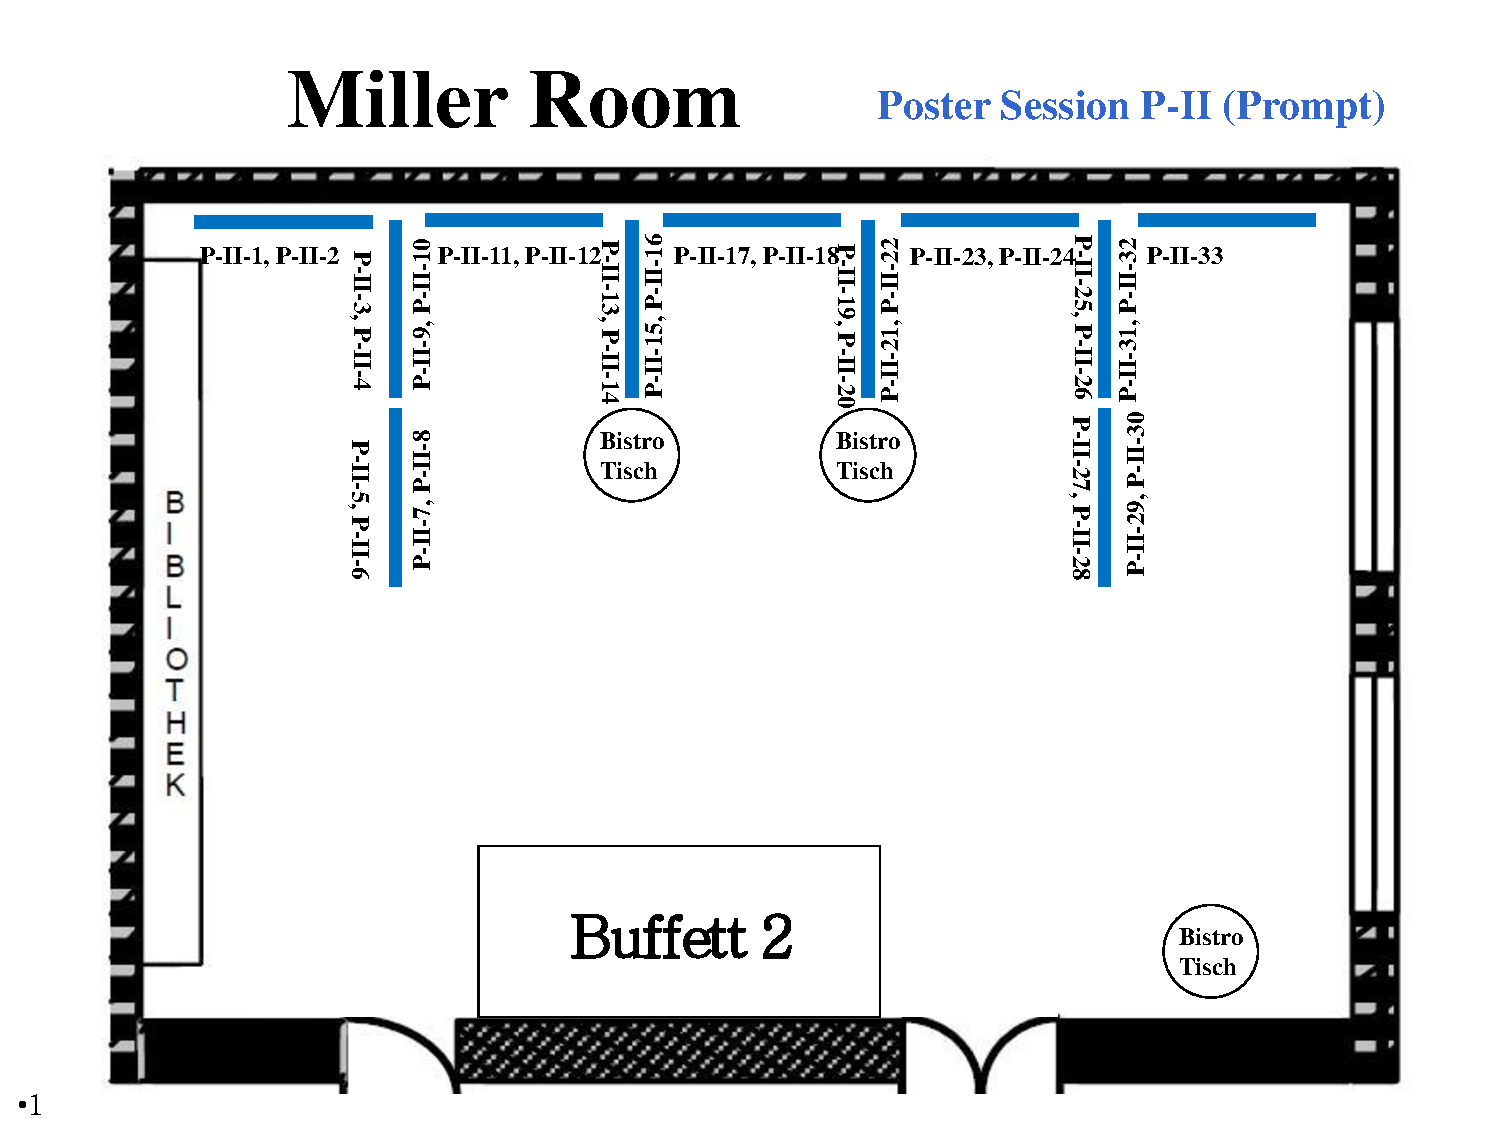
\includegraphics[scale=0.5]{pg_0001.pdf}

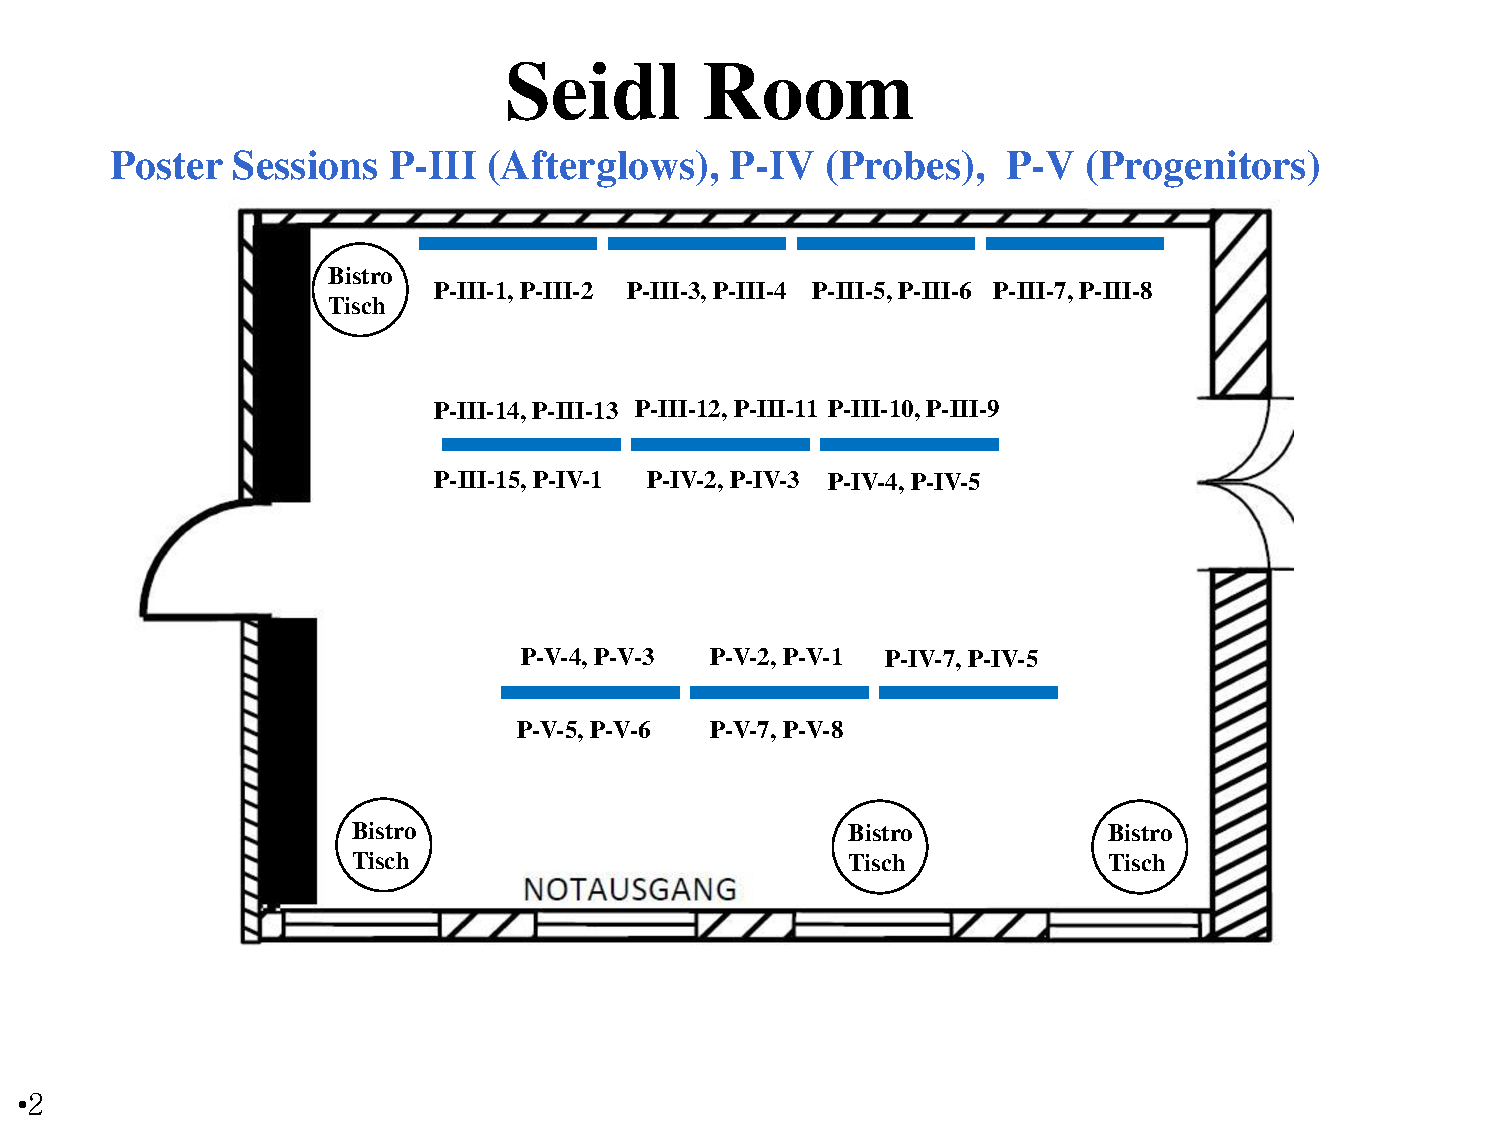
\includegraphics[scale=0.5]{pg_0002.pdf}

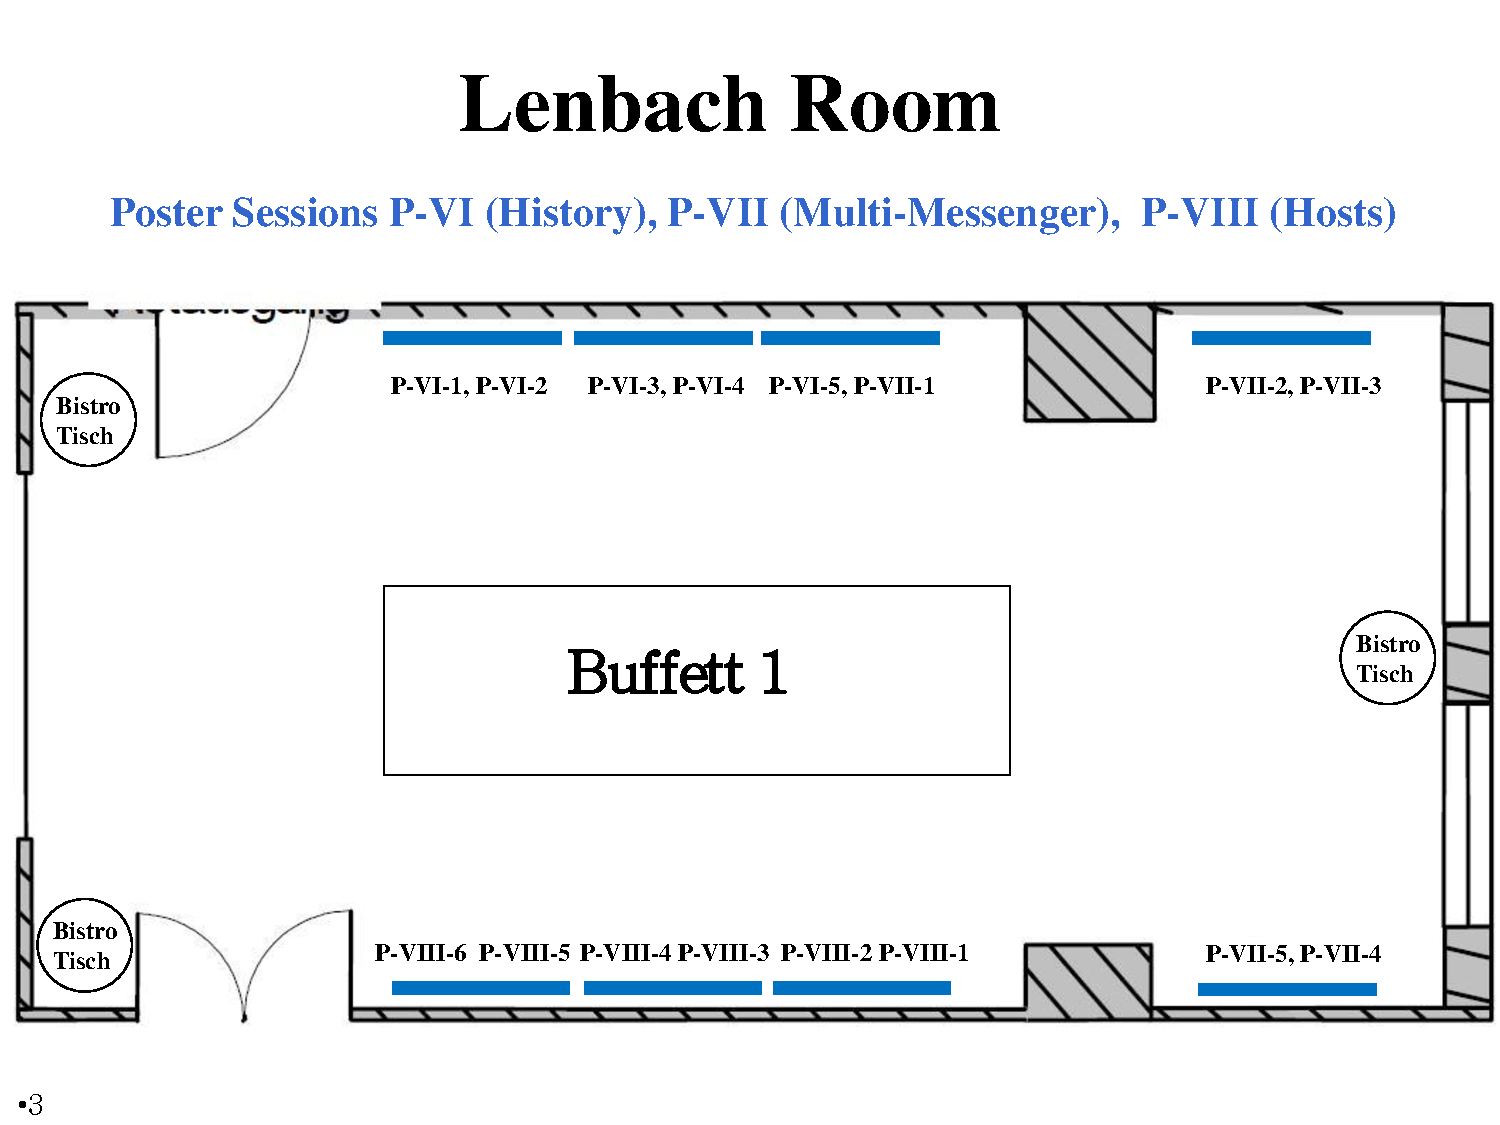
\includegraphics[scale=0.5]{pg_0003.pdf}


\end{document}
